\let\ActiveRetinaPrimitiveYear\year
\documentclass{ieeeaccess}
\let\ActiveRetinaAccessYear\year
\let\year\ActiveRetinaPrimitiveYear
% Define the class accent before pgfplots loads xcolor, avoiding a broken spot-color resource.
\definecolor{accessblue}{cmyk}{1,.37,0,.39}
\usepackage{cite}
\usepackage{amsmath,amssymb,amsfonts,booktabs,tabularx,array,url,graphicx,pgfplots}
\let\year\ActiveRetinaAccessYear
\pgfplotsset{compat=1.18}
\usepackage[T1]{fontenc}
\usepackage{microtype}
\newcommand{\system}{ActiveRetina-RC}
\title{Selection History and Operating-Point Evaluation in Diabetic Retinopathy Screening: A Retrospective Evidence Audit}
\history{Date of publication xxxx 00, 0000, date of current version xxxx 00, 0000.}
\doi{10.1109/ACCESS.2017.DOI}
\vol{XX}
\year{2026}
\author{\uppercase{Burak Ata Aksu}}
\corresp{Corresponding author: Burak Ata Aksu (e-mail: bataaksu1@gmail.com).}
\markboth{Aksu: Selection History in DR Screening}{Aksu: Retrospective Evidence Audit}
\begin{document}

\begin{abstract}
We audited two non-comparable evidence objects in diabetic-retinopathy (DR) screening: a frozen raw-image classifier evaluated at a development-selected threshold and a separate, exposed precomputed-score policy replay. On the MMRDR source-designated ultra-widefield test partition, the frozen ResNet-50 detected 1,283/1,288 referable images (99.61\%; image-level Wilson 95\% confidence interval [CI], 99.09--99.83\%) but cleared only 262/1,309 nonreferable images (20.02\%; 95\% CI, 17.94--22.27\%), with five false-negative images. At the same threshold, model-selection sensitivity and specificity were 100.00\% and 20.50\%, respectively: the zero-miss condition failed to transfer, while specificity changed by -0.48 percentage points. Two positive test images had byte-identical copies in model-fit data, and the available exports do not support a patient-level independence audit. Post-hoc test-score analysis found ROC-AUC 0.917 and 9.40\% specificity at 100\% observed sensitivity; this is not a deployable threshold. Separately, deterministic replay of a precomputed-score policy on an exposed 981-eye cohort yielded 70.13\% specificity (270/385) with no observed referable or ungradable eye clearances. Patient-grouped calibration of the fixed recipe yielded 69.61\% (268/385; difference $-0.52$ points; conditional patient-cluster bootstrap 95\% CI, $[-1.31,0.00]$). Among 596 referable-or-ungradable eye records, three decisions changed from REFER to CLEAR under grouped calibration (3/596 versus 0/596; paired eye-level missed-required-eye-rate difference +0.50 percentage points, conditional patient-cluster bootstrap 95\% CI, 0.00--1.17). The intervals condition on fixed decisions and do not adjust for selection. This is a bounded evidence audit, not a new model, risk guarantee, or clinical-validation claim.
\end{abstract}

\begin{keywords}
Diabetic retinopathy, fundus imaging, patient-level validation, model selection, score fusion.
\end{keywords}
\titlepgskip=-21pt
\maketitle

\section{Introduction}
\IEEEPARstart{D}{eep} learning has achieved high discrimination for diabetic retinopathy (DR) in retinal photographs, including large-scale and multiethnic evaluations \cite{gulshan2016,ting2017,abramoff2018,bellemo2019}. For screening, however, discrimination is only part of the problem. A system must make a thresholded decision, and the apparent operating point can depend strongly on how score normalization and thresholds were selected relative to the evaluation cases. In multi-source medical pipelines, quantifying the gap between deterministic replay and patient-grouped internal development estimation matters because repeatedly tuning score channels, calibration, and thresholds on the evaluation cohort can inflate the apparent operating point even when the final rule is replayed perfectly.

We examine two distinct evidence objects rather than compare them as competing models. The first is a frozen ImageNet-pretrained ResNet-50 classifier evaluated at a development-selected threshold on the source-designated ultra-widefield (UWF) test partition of the Multi-Modal Retinal images for in-depth DR analysis (MMRDR) dataset. The second is a precomputed-score policy replayed on a repeatedly inspected, multi-source 981-eye cohort. The former measures raw-image inference at a locked threshold; the latter reproduces actions from supplied component scores. Their inputs, cohorts, and selection histories differ, so their percentages are not a head-to-head comparison.

The frozen MMRDR rule detected 1,283/1,288 referable test images but cleared only 262/1,309 nonreferable images, yielding 99.61\% sensitivity and 20.02\% specificity with five false-negative clearances. A post-hoc exact-byte audit found two positive test images duplicated in model-fit data; this overlap and the absence of patient identifiers limit the partition's independence. In the separate exposed score cohort, deterministic replay yielded 70.13\% specificity (270/385), while patient-grouped calibration yielded 69.61\% (268/385) and three referable or ungradable clearances. The grouped interval is conditional on fixed decisions and does not account for prior cohort-wide exploration or selection. These results motivate an audit of how operating-point evidence changes with evaluation procedure; they do not establish a transferable risk guarantee or clinical performance.

The general concern is selection, not this project alone. A screening workflow may choose a high-sensitivity operating point and report specificity at that threshold. If model variants, score channels, calibration rules, or safety margins are repeatedly inspected on the same patients, the nominally conservative zero-miss constraint itself becomes a selection target. Patient-grouped cross-validation can estimate a specified procedure, but it cannot erase cohort-wide exposure that occurred before folds were created. We therefore distinguish deterministic replay, internal development estimation under patient-grouped procedures, and independent external testing on a cohort not used for model or analysis decisions.

Our retrospective questions are: (1) does a development-selected threshold retain its miss--specificity behavior on the dataset's source-designated test partition under a fixed-threshold analysis; (2) how do deterministic replay and patient-grouped or nested development estimates differ on the previously inspected multi-source cohort; and (3) how sensitive are grouped-selection outcomes to candidate-panel size and patient split? These questions describe the analyses conducted; they were not prospectively registered, and the results do not support population-level hypothesis tests \cite{openaiChatGPT}.

\subsection{Contributions}
\begin{enumerate}
\item A raw-image referable-DR classifier based on an ImageNet-pretrained ResNet-50 with a frozen encoder and a trained six-grade linear head; the exact operating-point selection rule and training/development split are described.
\item A one-time, frozen-threshold evaluation on 2,597 images from the MMRDR-UWF official test partition, with the confusion counts, specificity interval, five false-negative clearances, and limits of row-level inference reported explicitly.
\item A paired five-seed candidate-panel audit and patient-grouped development analysis on a different, repeatedly inspected 981-eye multi-source score cohort.
\item An exact replay specification for the historical 70.13\% score policy, kept separate from raw-image model inference.
\item Failure analyses of additional image-model and transfer experiments, including a ConvNeXt-Tiny development comparator whose test partition was not evaluated.
\item A reproducible controlled simulation, with an identical-candidate negative control, that demonstrates the effect of candidate-panel search on an empirical zero-miss operating point under stated distributional assumptions.
\end{enumerate}

The contributions are audit and measurement contributions, not a claim of architectural novelty. In particular, this study does not introduce a new retinal representation, risk-control theorem, dataset, or prospective workflow. Recent DR studies already compare decision strategies at fixed sensitivity and evaluate threshold transfer across datasets; we therefore do not claim either question as new in isolation. Our methodological contribution is an applied selection-history map: each reported result is linked to its input unit, outcome-dependent choices, partition/overlap status, and permissible inference. We apply this map to exposed deterministic replay, patient-grouped internal development estimates, candidate-panel-by-split sensitivity, post-hoc test-score diagnostics, a synthetic mechanism experiment, and a separate frozen raw-image test. The map is an auditable reporting device for this case, not a validated general-purpose bias correction. Independent replication remains necessary.

\section{Related Work}
\subsection{Automated DR Screening and Dataset Benchmarks}
Automated DR grading has been studied from benchmark datasets through large multiethnic cohorts and prospective primary-care settings \cite{gulshan2016,ting2017,abramoff2018,bellemo2019}. These studies establish that fundus-image classifiers can reach clinically relevant discrimination under defined acquisition and reference-standard conditions. Their claims are not directly interchangeable: populations, cameras, gradability rules, disease thresholds, adjudication, and clinical workflow differ. The present study is not a head-to-head reimplementation of these systems. It evaluates one frozen image-classification operating point on an official held-out dataset partition and separately audits a multi-source score policy whose normalization and thresholds were derived from its reported cohort.

A 2026 systematic review and meta-analysis of regulator-approved fundus-based systems synthesized 82 studies, 887,244 examinations, 25 devices, and 28 countries. Its pooled sensitivity/specificity estimates were 0.93/0.90 per patient and 0.92/0.93 per eye; meta-regression identified disease threshold, national-income level, image gradability, pupil dilation, reference standard, and diagnostic criteria as factors explaining between-study heterogeneity \cite{wang2026approveddr}. These estimates concern a distinct evidence base and are not a comparator for this study. They reinforce why operating points should be reported with their cohort, acquisition conditions, endpoint, and selection history; this audit neither estimates real-world performance nor explains the review's heterogeneity.

The three-source development pool combines the Diabetic Retinopathy Dataset (DDR), the Deep Diabetic Retinopathy Image Dataset (DeepDRiD), and the Diabetic Retinopathy Two-field image Dataset (DRTiD). DDR provides a large, multi-task fundus benchmark with grading and lesion annotations \cite{ddr}. DeepDRiD was constructed around grading and image-quality estimation and includes multiple views per eye in its regular fundus subset \cite{deepdrid}. DRTiD was introduced for two-field DR grading, motivating paired-field modeling rather than assuming a single image is always sufficient \cite{drtidpaper}. Dataset names alone do not make a pooled cohort homogeneous. The study retains source identity in both score calibration and reporting, and does not interpret the pooled specificity as a target-clinic estimate.

Recent multiview DR work develops the diagnostic model itself: CrossFiT models cross-field correspondence in two-field images; a later four-view method adds cross-view spatial alignment and vessel reinforcement; and an AAAI 2026 method addresses incomplete-view inputs through self-supervised inter- and intra-view restoration \cite{drtidpaper,lin2025multiview,wu2026incompletemv}. These are architectural and representation-learning contributions. The present work asks a different question: how threshold and candidate selection affect zero-observed-miss operating-point transfer and its auditability. It neither reproduces nor benchmarks those multiview methods, and its exposed score-policy cohort cannot establish their relative clinical performance.

MMRDR includes color fundus photographs (CFP), optical coherence tomography (OCT), and ultra-widefield (UWF) images with distinct labels and partitioning \cite{mmrdr,mmrdrdata}. The primary model analysis uses UWF only. Its official held-out test partition is evaluated after the checkpoint and threshold were frozen; it is not an external-dataset or prospective evaluation. CFP and UWF filenames were not treated as paired patient-eye records.

\subsection{Selective Prediction, Risk Control, and Operating Points}
Selective classification studies predictions accompanied by a reject or defer option, with coverage and selective risk reported jointly \cite{geifman2017,selectivenet}. In a medical workflow, referral is not necessarily a reject in the algorithmic sense: it may be the intended safe action for a positive or uncertain case. Here, every record is assigned one of two actions, CLEAR or REFER. We call the proportion assigned either action binary action assignment, reserving ``coverage'' in the product sense for a clinically validated prediction pathway. A 100\% binary action assignment rate in a finite replay does not demonstrate that all images can be diagnosed safely.

Directly relevant DR work now evaluates decision rules as part of the screening system rather than treating the classifier score as the whole product. On 5,270 EyePACS images (1,366 labeled as DR), Jena and Rayguru compare five strategies at prespecified sensitivity targets; at 95\% sensitivity, their best single-model strategy reaches 17.5\% specificity, while a weighted ensemble at 90\% sensitivity reduces unnecessary referrals by nearly 25\% relative to the single-model 95\% setting \cite{jena2026}. This prior result makes clear that neither fixed-sensitivity policy comparison nor the high-sensitivity/specificity trade-off is novel by itself. Our work does not reproduce their models or compare those operating points head to head. Its distinct, narrower question is how a historically reused retinal pipeline's operating-point evidence changes across deterministic score replay, patient-grouped and nested procedures, candidate-panel sensitivity, and a separate frozen image-model test. The EyePACS and MMRDR cohorts, label definitions, inputs, model outputs, and estimands differ; the reported numbers are contextual only and cannot be ranked against one another.

Finite-sample risk control and conformal methods can provide guarantees only when their assumptions and split protocol are satisfied; an empirical threshold chosen by inspecting the evaluation outcomes does not acquire a guarantee by being called conservative \cite{vovk2005,angelopoulos2021,angelopoulos2024}. A zero observed miss count is a sample outcome. It is not the proposition that the future missed-disease probability equals zero. If a fixed classifier has no misses in a sample, uncertainty about its population risk remains, and tuning the classifier or threshold on that same sample invalidates a naïve fixed-rule interpretation.

\subsection{Selection Bias and Structured Validation}
Repeated selection among models or thresholds can produce optimistic performance estimates even when each individual candidate is evaluated with a conventional metric \cite{cawley2010,varma2006}. Nested cross-validation addresses one part of this problem by separating the inner selection step from outer evaluation. Grouped folds address another: images from the same patient should not straddle training/calibration and evaluation partitions when patient-level generalization is the intended estimand. Similar grouping principles apply to spatial, hierarchical, and repeated-measures data \cite{roberts2017}.

Diagnostic-accuracy work has also addressed inference after choosing among multiple candidate tests and cutpoints. Westphal and Zapf compare family-wise-error procedures for this setting, including bootstrap-based methods \cite{westphal2024}. That work is closer to the threshold-selection problem than general machine-learning validation references, and it rules out presenting multiplicity-aware diagnostic inference as a new contribution here. We do not implement, extend, or empirically compare those procedures. Instead, this manuscript audits a retrospective retinal pipeline whose score references and policy candidates were iteratively inspected on a shared cohort, and documents how its zero-observed-miss operating point changes across replay, patient-grouped development analyses, nested selection, and a separate frozen image-model test. The result is a bounded case study of evidence provenance and selection sensitivity, not a general correction for selection bias.

A 2026 factorial radiomics study already decomposes cumulative analytical leakage using simulations and TCIA data \cite{garciahidalgo2026}. In its pure-noise simulation with 50 cases and 1,000 features, the fully leaked pipeline reached AUC 1.000 while the properly nested reference was 0.493; it also examined real TCIA radiomic features. We therefore do not claim to introduce medical-imaging leakage audits or the general principle of nesting analytical choices. Our narrower question concerns candidate-panel-by-partition behavior for a zero-miss operating point in a multi-source retinal score pipeline. The evidence here is a project-specific sensitivity analysis, not a new general method.

Diagnostic cutpoint selection and repeated test reuse also have direct prior art. Leeflang et al. quantified optimism from data-driven cutoff selection and compared approaches intended to reduce it; Westphal and Zapf studied inference for diagnostic accuracy when multiple tests or cutpoints are compared \cite{leeflang2008,westphal2024}. In a different modality and post-market setting, Yamanaka et al. simulated repeated reuse of the same test set while selecting and integrating bone-scintigraphy models, observed performance bias, and assessed a differential-privacy-based bias-reduction method \cite{yamanaka2026}. These studies rule out novelty claims for cutoff optimism, multiple-cutpoint inference, or test-set reuse as general phenomena. ActiveRetina does not implement those correction methods. Its bounded contribution is a retrospective DR case study that reconciles a historical score replay, patient-grouped and nested analyses, candidate-panel sensitivity, and a distinct fixed-threshold image-test analysis; the synthetic experiment isolates one stated mechanism and is not evidence that it caused the project results.

These safeguards do not undo prior full-cohort inspection. In this project, the component score library and cohort had already been examined, and candidate families had been developed in response to observed results. Consequently, patient-grouped and nested estimates in this paper are more informative than the full-cohort replay about within-cohort selection behavior, but they are not a pristine confirmatory experiment. This distinction is central to the manuscript's interpretation.

\subsection{Domain Shift and Multisource Learning}
Fundus datasets differ in camera response, field of view, compression, illumination, patient mix, disease prevalence, grading, and image quality. Domain generalization work explicitly studies performance on distributions not represented during training, including DR benchmarks \cite{galappaththige2024}. Multisource training can help when the sources provide complementary support, but indiscriminate pooling can also shift the learned decision boundary away from the target source. Ophthalmic foundation models such as RETFound provide broadly pretrained representations but still require target-domain testing \cite{retfound}. The MMRDR experiment below tests this operationally: an auxiliary CFP source and an ophthalmic foundation-model representation were evaluated on a fixed UWF development validation split, and neither was presumed beneficial in advance.

Operating-point transfer in DR has also been studied directly. Bhuiyan et al. report that an APTOS-selected threshold yielded 69.41\% sensitivity at high specificity on external IDRiD; target-domain calibration on a separate split raised the reported held-out operating point to 93.42\% sensitivity and 84.30\% specificity \cite{bhuiyan2026}. This prior work rules out any claim that the present study is the first DR analysis of threshold transfer. The present MMRDR analysis instead reports a frozen threshold on the dataset's official UWF partition, while the separate candidate-panel audit concerns a historically exposed multi-source score cohort. These designs answer different questions and are not comparative model evaluations; the two studies together reinforce that threshold performance must be described with its selection history and target domain.

Three recent studies further bound the novelty and interpretation of UWF results. Li et al. evaluated ophthalmic foundation models across Danish and Greenlandic UWF populations; external discrimination was lower than within-population performance, and calibration remained poor even after sequential adaptation \cite{li2026uwf}. A separate medRxiv preprint compared generalist and ophthalmic foundation models on BRSET and mBRSET, likewise reporting external discrimination loss and residual calibration concerns \cite{li2026mbrset}. Poyrazer et al. compared frozen MedSigLIP, RETFound, and EfficientNet-B0 encoders with a shared trained head on APTOS and zero-tuning MESSIDOR-2; similar development AUCs separated under external testing, and development temperature scaling did not resolve external calibration error \cite{poyrazer2026frozen}. Their study directly addresses frozen-representation transfer and calibration, so we make no claim to introduce either question. Our MMRDR classifier instead uses a frozen ImageNet ResNet-50 and a study-trained six-logit head; this manuscript's distinct contribution is an audit of operating-point provenance and selection history alongside its unfavorable, fixed-threshold within-dataset test. The cited studies use different cohorts, endpoints, models, and estimands and are not performance comparators. Collectively, they make it especially important not to infer clinical transfer from our within-dataset result or from score ranking alone.

Sheng et al. provide another recent example: ORDER-DR reports external evaluation of DR severity grading and referable-risk stratification, with threshold selection and external testing treated as distinct stages \cite{sheng2026orderdr}. This reinforces the need to state whether a threshold was transported unchanged or adapted using target-domain data. Our frozen MMRDR threshold is a within-dataset held-out evaluation, not external transfer; our score-policy replay is exposed and cannot estimate transfer at all. We thus position the two results as different evidence boundaries, not as evidence that our policy is more robust or that ORDER-DR's model is a direct baseline.

The broader operating-point problem is not unique to ophthalmology. Abdikenov et al. recently reported near-zero specificity at a conventional threshold in cross-dataset breast-ultrasound classification despite nontrivial discrimination, and studied source-confounding and training interventions across public datasets \cite{abdikenov2026}. This is adjacent evidence for the general importance of fixed-threshold reporting, not evidence for the same mechanism in retinal imaging. We do not claim that operating-point collapse, cross-dataset threshold failure, or multi-source selection bias is new across medical imaging. Our narrower contribution is a retrospective retinal audit that keeps an exposed score-policy replay, patient-grouped development estimates, candidate-panel sensitivity, and a separate frozen within-dataset image test as distinct evidence objects. The ultrasound study does not evaluate retinal images or our candidate-panel protocol, while our experiments do not reproduce its intervention results or establish a cross-modality law.

\subsection{Reporting Guidance and Positioning}
The Checklist for Artificial Intelligence in Medical Imaging (CLAIM) and its 2024 update provide reporting prompts. The Transparent Reporting of a multivariable prediction model for Individual Prognosis Or Diagnosis--Artificial Intelligence (TRIPOD+AI) statement covers clinical prediction-model reporting \cite{claim,claim2024,tripodai}. The CLAIM update discourages the ambiguous term ``validation'' and recommends describing internal and external testing; accordingly, this manuscript uses ``internal model-selection subset'' for the MMRDR development carve-out and reserves ``external testing'' for a genuinely independent cohort. Where ``validation'' remains, it identifies the dataset's or source artifact's own partition label, not independent clinical testing. We use these guidelines as reporting aids rather than claiming checklist compliance. The current study lacks several elements expected for a clinical diagnostic accuracy paper, including independent sites, prospective workflow, complete raw-image inference provenance, and clinician adjudication. We make those absences explicit in the claim ledger and conclusion \cite{openaiChatGPT}.

\section{Methods}
\subsection{Cohort and Label Definitions}
The replay manifest contains 981 eye-level records: 625 DDR, 106 DeepDRiD, and 250 DRTiD. Harmonized labels comprise 385 gradable nonreferable eyes, 463 gradable referable eyes, and 133 ungradable cases. Gradable referable disease follows the project convention of grades 2--4; ungradable cases are reported separately and are intended to be referred \cite{ddr,deepdrid,drtidpaper}. The cohort was repeatedly inspected during model and threshold development. It is therefore an exposed development cohort, not a sealed test set.

The master manifest has 928 unique patient identifiers for 981 eye records. DDR contributes 625 records from 625 patient IDs; DeepDRiD contributes 106 eyes from 53 patients; DRTiD contributes 250 records from 250 patient IDs. The distinction between eye and patient is material: two eyes from one DeepDRiD participant remain together in each patient-grouped partition. Pooled metrics give each eye one count, so the aggregate is case-weighted rather than patient-weighted or population-standardized.

The binary boundary follows the project convention: gradable grades 0--1 are nonreferable and grades 2--4 are referable. Records without a usable grade or not meeting a source gradability rule are tracked as ungradable rather than mapped to negatives. In the audited score policy, ungradable cases are required to receive REFER; they do not enter the gradable-negative specificity denominator. This is an analysis convention, not a claim that the source datasets use identical clinical gradability standards.

The source-specific composition and replay counts are reported in Table~\ref{tab:source}. The pooled denominator is the sum of source-specific gradable nonreferable eyes; it is not a patient-standardized estimate.

The primary raw-image experiment uses MMRDR ultra-widefield (UWF) photographs. The official training pool comprised 7,807 images; a stratified image-level 15\% carve-out assigned 1,172 to model and threshold selection, leaving 6,635 fit images. For clarity, we call this the internal model-selection subset throughout; references to a source file's ``validation'' partition describe its provenance and do not mean independent external testing. The frozen candidate was evaluated on the source-designated UWF test partition (2,597 images). A local integrity audit joined the prediction export to all test-manifest rows by unique image identifier and found exact agreement in grade and referable-disease label. A second audit matched test images to the source UWF annotation CSV and verified grade agreement. The source CSV contains image, grade, lesion, and laterality fields but no patient-link key. Although the derived manifest schema includes patient and eye identifier columns, all 2,597 values in each column are empty; the prediction export also omits these identifiers. Thus, the local files do not permit patient-clustered uncertainty estimates or independent verification of patient-level separation.

We additionally computed SHA-256 hashes over original image bytes for all 10,404 images in the local UWF manifest, joining duplicate groups to official partitions, the cached-feature fit/model-selection split, and frozen test predictions. Eight exact-duplicate groups (eight rows beyond one copy per group) were found: six were confined to a single official split and two crossed the official train/test boundary. Both training copies of the cross-split duplicates were in the internal model-fit split; no exact duplicate group crossed the internal fit/model-selection boundary. Both duplicated test rows were referable and were referred by the frozen classifier. The primary counts on all test rows are 1,283/1,288 true positives, five false negatives, 262/1,309 true negatives, and 1,047 false positives. Excluding the two known duplicate test rows post hoc yields 1,281/1,286 true positives and the same 262/1,309 true negatives; specificity remains 20.02\%. The unchanged result shows that these two exact copies do not account for low specificity or the five observed misses, but this filtered analysis cannot restore a clean test because the outcomes were already inspected. This byte-level procedure does not detect recompressed or transformed near-duplicates and cannot detect other patient-level overlap. The dataset description designates its official UWF test split as patient-level, but that property cannot be independently audited from the local rows \cite{mmrdr,mmrdrdata}. The MMRDR descriptor identifies OIA-DDR as the source of its CFP subset; no CFP-to-UWF join was made from numeric filename suffixes because matching suffixes alone do not establish same-eye correspondence \cite{mmrdr}. A subsequent multi-source fine-tune combined DDR, DeepDRiD, DRTiD, and IDRiD training images \cite{idrid}, but a later audit found that every eye in the historical 981-eye reference appeared in its validation rows; that experiment is exposed with respect to the reference and is not the primary test result.

\subsection{Image Classifier and Operating-Point Selection}
One implementation detail affects interpretation of the classifier score: the six-logit head has outputs for grades 0--5, while this experiment contains categorical labels only for grades 0--4, and the referable score aggregates logits 2--5. The grade-5 logit therefore has no direct grade-5 categorical examples. It may still receive indirect gradients from binary referable, pairwise-ranking, and hard-boundary losses, all of which act on the aggregate referable score. Because the checkpoint is unavailable, its contribution cannot be isolated; we do not infer the direction or magnitude of any effect on the reported test metrics.
The evaluated image classifier uses the \path{resnet50.a1_in1k} ResNet-50 implementation with ImageNet-1K initialization and 224-by-224 RGB inputs. The evaluation transform uses bicubic resizing, a centered crop at 95\% of the scaled image, and ImageNet channel normalization (means 0.485/0.456/0.406; standard deviations 0.229/0.224/0.225). The convolutional encoder is frozen; cached 2,048-dimensional image features feed a trainable linear six-logit categorical head, giving 12,294 trainable parameters (including bias). Its output indices are 0--5, but the MMRDR-UWF rows used in this experiment have labels only at indices 0--4. The binary referable endpoint is grade $\geq2$. The deployed score is the log-sum-exp of logits at indices 2--5 minus the log-sum-exp at indices 0--1; thus index 5 contributes to the score despite having no MMRDR training examples with that class label. This is a pretrained-backbone classifier trained for this study, not a fully fine-tuned retinal foundation model.

Training uses only rows marked \texttt{train} in the official UWF training partition; the 1,172-image validation carve-out is image-level because exported patient identifiers are unavailable. The checked-in trainer defines a weighted multiclass cross-entropy on the grade index (its option is named \texttt{ordinal-weight}, but the loss does not encode distances between grades), binary referable-risk cross-entropy, pairwise ranking loss, and a hard-boundary loss emphasizing difficult positives and negatives around grades 1 and 2. The run card preserves checked-in defaults, not verified run-specific arguments; the original command line was not archived, so the exact loss coefficients used in this run are unknown. The selected checkpoint is epoch 20 of 26 recorded epochs. Its stored validation threshold is the minimum validation referable score, $-1.8022103309631348$ on the uncalibrated logit scale, a zero-observed-miss development rule; this threshold gave 572/572 validation positives detected and 123/600 negatives cleared. We recovered and hashed the development manifest (7,807 rows; 6,635 training and 1,172 validation), cached feature file (7,807 by 2,048 float32 values), trainer, and feature-extraction source. The historical training summary records the architecture, selected epoch, trainable-parameter count, validation metrics, and threshold. The checkpoint file is absent from the current checkout; its previously recorded SHA-256 cannot now be reverified against the checkpoint bytes. The checkpoint, feature cache, source-model weight revision, and full run environment are not in the public package, so exact clean-clone inference and bit-for-bit retraining remain unavailable.

To test whether the recovered implementation and development cache could reproduce the recorded trace, we reran the checked-in trainer defaults using the hash-verified development inputs. At epoch 1, the historical trace records training loss 2.721 and zero-miss validation specificity 4.67\% (threshold $-1.350$); the reconstruction records loss 10.591 and specificity 0.50\% (threshold $3.802$). The reconstruction completed 11 validation epochs and stopped before checkpoint saving because pretrained backbone weights were unavailable locally. It did not read official-test inputs or outputs. This is a failed development-trace reconstruction, not a new model result; it leaves the cause unresolved among unrecorded run-specific arguments, runtime differences, and other missing provenance, and it does not alter the official-test result.

The primary fixed-threshold analysis used the official test partition with the frozen checkpoint and validation-selected threshold; no model, threshold, or preprocessing adjustment was made using test outcomes. Subsequent score-ranking and sensitivity-constrained frontier diagnostics were computed after inspecting the test export and are reported only as post-hoc descriptions. The test partition is therefore not untouched for future confirmation, even though these diagnostics did not alter the primary analysis. The official split is the dataset's internal held-out test rather than an external dataset or prospective clinical cohort. Since released rows contain no patient identifiers, reported confusion counts are image-level, and image-level uncertainty calculations cannot be interpreted as patient-clustered inference.

After the frozen result had been inspected, we conducted a secondary score diagnostic on the hash-verified prediction export. ROC-AUC was computed as the Mann--Whitney statistic with average ranks for ties; average precision grouped tied scores before updating precision and recall. For each stated minimum-sensitivity constraint, the diagnostic enumerated unique observed test scores and retained the point with greatest test specificity satisfying that constraint. This test-label-derived envelope is post-hoc and is reported only to distinguish ranking from thresholded utility; it is not a model-selection procedure, and no envelope cutoff is proposed for deployment. The script emits aggregate-only JSON. Because the export lacks patient IDs, we report no patient-clustered uncertainty for these diagnostics.

The MMRDR development-candidate comparison appears in Table~\ref{tab:mmrdr}; all rows use the same inspected image-level model-selection subset and are reported as development diagnostics. The frozen ResNet-50 head's official-test performance is reported separately as the primary image-model result.

\begin{table*}[t]
\centering
\caption{Composition and deterministic replay of the frozen 70.13\% policy. Specificity is computed only on gradable nonreferable cases.}
\label{tab:source}
\begin{tabular}{lrrrrrrrr}
\toprule
Dataset & Cases & Gradable nonref. & Gradable ref. & Ungradable & TN & FP & Misses & Specificity \\
\midrule
DDR & 625 & 206 & 286 & 133 & 134 & 72 & 0 & 65.05\% \\
DeepDRiD & 106 & 52 & 54 & 0 & 51 & 1 & 0 & 98.08\% \\
DRTiD & 250 & 127 & 123 & 0 & 85 & 42 & 0 & 66.93\% \\
\midrule
Pooled & 981 & 385 & 463 & 133 & 270 & 115 & 0 & 70.13\% \\
\bottomrule
\end{tabular}
\end{table*}

\subsection{Data Provenance and Source Harmonization}
The pooled reference table is an analysis manifest, not a newly collected prospective cohort. Source data remain governed by their original access terms and licenses; raw images are not redistributed. The source notices are not uniform: the MMRDR version-2 Figshare item displays CC BY 4.0 (\url{https://figshare.com/articles/dataset/MMRDR/29423747}); the DDR repository identifies its dataset materials as CC BY-NC-SA 4.0 while distinguishing MIT-licensed repository code (\url{https://github.com/nkicsl/DDR-dataset}); the DeepDRiD repository displays CC BY-SA 4.0 (\url{https://github.com/deepdrdoc/DeepDRiD}); and the DRTiD repository describes research-only, application-based access without displaying a standard dataset license (\url{https://github.com/FDU-VTS/DRTiD}) \cite{mmrdrdata,ddr,deepdrid,drtidpaper}. Because the MMRDR descriptor identifies OIA-DDR as the source of its CFP subset, the MMRDR item's displayed license is not treated here as a determination that upstream third-party CFP rights are cleared \cite{mmrdr,ddr}. These notices are reported as source metadata, not as a legal interpretation of every dataset component or a determination that pooled derived records may be redistributed. Accordingly, this manuscript releases no raw images or per-eye score/label rows, and the complete score replay is not reproducible from the public bundle. Dataset-specific identifiers are namespaced so that identical strings from different sources do not imply the same person. The public package supplies checksums for its aggregate audit artifacts and an MMRDR run card, but it does not include a complete record-level source-partition map or immutable snapshot identifiers for every source. Therefore, a clean clone can check the included aggregate summaries but cannot reconstruct the row-level cohorts, execute the score replay, or reproduce image inference. These omissions are explicit reproducibility limitations; this manuscript does not claim that its supplement completes the provenance trail.

The source studies report different ethics and consent procedures. The MMRDR data-descriptor reports approval by the Institutional Review Board of Qingdao Eye Hospital of Shandong First Medical University (QingYanLunShen[2024] No. 41) and waiver of informed consent for its retrospective collection; the DeepDRiD challenge study reports approval by the Ethics Committee of Shanghai Sixth People's Hospital and that participant informed consent was obtained \cite{mmrdrdata,deepdrid}. These statements describe the original source studies only. They do not establish the ethics determination, consent basis, or scope applicable to the present secondary analysis, which must be documented separately by the author. This manuscript does not infer source-study procedures for DDR or DRTiD from the procedures reported for MMRDR or DeepDRiD.

The roles are distinct. The 981-eye pool is an exposed reference for the original 70.13\% score policy. MMRDR UWF training and internal model-selection subsets support model fitting and threshold selection, while the official UWF test partition provides one frozen held-out evaluation. This is stronger than a reused model-selection result but remains internal to one dataset and has no exported patient IDs for an independent grouping audit. The larger image count does not by itself imply population representativeness or clinical validity.

For the candidate names below, DINO denotes ``self-distillation with no labels''; the candidate uses the \path{vit_base_patch16_224.dino} base Vision Transformer encoder (patch size 16, input size 224). HGB denotes the HistGradientBoosting classifier, and RBF-SVM denotes a support-vector machine with a radial-basis-function kernel \cite{dino}.

\begin{table}[t]
\centering
\caption{MMRDR-UWF development candidates with retained aggregate run summaries. Each zero-miss threshold was selected on the same inspected internal model-selection subset; entries are development diagnostics, not external testing.}
\label{tab:mmrdr}
\begin{tabularx}{\columnwidth}{>{\raggedright\arraybackslash}Xrr}
\toprule
Candidate & TN/600 & Specificity \\
\midrule
ResNet-50 cached UWF head & 123 & 20.50\% \\
DINO frozen UWF head & 148 & 24.67\% \\
DINO hard-head UWF candidate & 86 & 14.33\% \\
ResNet+DINO feature stack, HGB & 151 & 25.17\% \\
RETFound-EyePACS features, HGB & 1 & 0.17\% \\
RETFound-EyePACS features, RBF-SVM & 60 & 10.00\% \\
RETFound-EyePACS features, logistic head & 63 & 10.50\% \\
Internal reference rank fusion & 202 & 33.67\% \\
Reference + 25\% RETFound-logistic rank & 207 & 34.50\% \\
\bottomrule
\end{tabularx}
\end{table}

\subsection{Why the Cohort Roles Are Not Interchangeable}
The three-source replay audits a policy whose component outputs exist for DDR, DeepDRiD, and DRTiD. The MMRDR experiment asks whether representations and heads transfer to ultra-widefield images under a separate model and validation-selection procedure. It does not validate the 70.13\% policy: it uses different inputs and model outputs, and the exact patient overlap between datasets cannot be established from the available exports. Conversely, the 981-eye replay does not validate the MMRDR candidates. We report them in separate tables and do not form a synthetic combined cohort by concatenating their metrics.

An initial numeric filename join between MMRDR CFP and UWF was discarded after an audit showed that equal suffixes did not establish eye-level correspondence. The final manifest treats CFP as auxiliary training data and UWF as the target development source. This correction prevents a false paired-image signal from entering either model training or evaluation. The rejected join is documented as a data-integrity failure, not as a result.

\subsection{Frozen Source-Conditional Policy}
For component $m$, source $d$, score $z$, and stored sorted reference vector $\mathcal{R}_{m,d}$ of length $n_{m,d}$, define the percentile midrank
\begin{equation}
 r_{m,d}(z)=\frac{L_{m,d}(z)+R_{m,d}(z)+1}{2n_{m,d}},
\label{eq:midrank}
\end{equation}
where $L_{m,d}(z)=\#\{x\in\mathcal{R}_{m,d}:x<z\}$ and $R_{m,d}(z)=\#\{x\in\mathcal{R}_{m,d}:x\le z\}$. The added one-count offset gives the average one-based rank for ties; this exact convention is part of deterministic replay. Source-specific scores are
\begin{equation}
\begin{aligned}
s_{\mathrm{DDR}} &= 0.50r_{\mathrm{aptos}}+0.10r_{\mathrm{ordinal}}\\
&\quad +0.40r_{\mathrm{audit}},\\
s_{\mathrm{DeepDRiD}} &= 0.20r_{\mathrm{ordinal-quality}}\\
&\quad +0.40r_{\mathrm{source-balanced}}+0.40r_{\mathrm{fundus}},\\
s_{\mathrm{DRTiD}} &= 0.72r_{\mathrm{rank-pair}}\\
&\quad +0.08r_{\mathrm{fundus-margin}}+0.20r_{\mathrm{geometry}}.
\end{aligned}
\label{eq:source-scores}
\end{equation}
The channel symbols in \eqref{eq:source-scores} denote the component ranks from \eqref{eq:midrank}; their names abbreviate the source-specific channels listed in Section III-B. The policy returns REFER when $s_d$ is at or above the source-specific threshold: 0.22224 (DDR), 0.435849 (DeepDRiD), and 0.34496 (DRTiD). The DDR rule additionally refers when its quality score is at least 0.0018599. Otherwise, the action is CLEAR. Both the empirical score-reference vectors and these thresholds were derived from the inspected cohort. They are disclosed for deterministic replay, not proposed as portable clinical cutoffs.

The evaluator consumes precomputed model outputs. It is not a single raw-image model, and the exact component checkpoints plus preprocessing contracts are not all bundled in the present repository. Thus, ``100\% action assignment'' denotes a deterministic binary action for each supplied feature record; it does not establish raw-image product readiness.

\subsection{Rank Fusion and Threshold Semantics}
The midrank in \eqref{eq:midrank} is implemented with left- and right-sided insertion positions in the sorted reference vector. Substituting a library percentile function without matching this boundary and tie convention can alter decisions. Each source has its own reference support, so identical raw component scores can map to different ranks across sources.

Let $\boldsymbol{w}_d$ be the nonnegative three-channel fusion weight vector for source $d$, with entries summing to one. The fused score is $s_d=\boldsymbol{w}_d^\top\boldsymbol{r}_d$, consistent with the source-specific expansions in \eqref{eq:source-scores}. For DDR, an additional quality override applies. The decision rule is
\begin{equation}
 a_i=\begin{cases}\mathrm{REFER},&s_{d(i)}\ge t_{d(i)}\;\text{or}\;q_i\ge q_0\text{ for DDR},\\
 \mathrm{CLEAR},&\text{otherwise},\end{cases}
\label{eq:decision}
\end{equation}
where $q_i$ is the stored quality signal and $q_0$ is the override threshold. The complete policy is thus a composition of pretrained or independently trained component systems, empirical normalization, weighted fusion, and threshold logic; it is not one end-to-end model trained under a unified loss.

Equation~\eqref{eq:decision} is the deterministic implementation contract evaluated in the replay; it is not a newly fitted or clinically validated decision rule.

The rank reference vectors were constructed from the same inspected records used to report replay performance. This transductive reuse is explicitly disclosed because the normalization support can encode the evaluation cohort's score distribution. A future frozen evaluation must fit these vectors on development patients only, then serialize them with model weights, image preprocessing, score ordering, thresholds, and quality rules. A threshold alone is not a complete model artifact.

\subsection{Endpoints}
Specificity is
\begin{equation}
\mathrm{Sp}=\frac{\mathrm{TN}}{N_{\mathrm{nonref,gradable}}},
\label{eq:specificity}
\end{equation}
where a true negative is a gradable nonreferable eye assigned CLEAR. A false-negative clearance is a gradable referable eye assigned CLEAR. We separately count ungradable clearances. Binary action assignment is the fraction of all records assigned either CLEAR or REFER. It is not equivalent to an independently validated diagnostic coverage rate.

Equation~\eqref{eq:specificity} defines the denominator used for every reported specificity; ungradable records are tracked separately and are not included in it.

For the strict operating-point summaries, a ``missed required eye'' is a gradable referable eye assigned CLEAR or an ungradable eye assigned CLEAR. We report these as eye/image-record counts, not patient-level outcomes; the two types are counted separately when artifacts allow. Specificity is calculated only among gradable nonreferable eyes; referring ungradable eyes does not change its denominator. In this replay, zero observed missed required eyes means all 463 gradable referable and 133 ungradable eye records received REFER.

We distinguish (i) manifest completeness, the fraction of cohort rows present in the scorer; (ii) action assignment, whether the policy emits CLEAR or REFER for each supplied score row; and (iii) product image coverage, whether an end-to-end implementation can ingest supported raw images and yield a valid clinical output. Only (ii) is measured as 100\% in the replay. It must not be reported as 100\% product coverage.

Exploratory policy selection used a lexicographic objective: minimize observed positive clearances first, then maximize true negatives, while assigning every scored row a binary action. This is an empirical development objective, not an expected-utility function. It does not account for site-specific referral burden, patient-level outcomes from paired eyes, or a prespecified finite-sample upper bound on missed-disease risk.

\subsection{Selection-history evidence map}
For each analysis object, we recorded four fields: (1) input and analysis unit (raw image, precomputed score row, or generated observation); (2) outcome-dependent choices, including fitting, checkpoint/candidate selection, score normalization, and threshold choice; (3) partition and identity evidence, including whether patient grouping was observed, verified, or unavailable; and (4) the narrowest inference supported by that history. We assigned an evidence class from these fields rather than from the metric value or the label ``test.'' Exact replay of the same records supports implementation consistency only. A fold-held estimate remains internal development evidence when the cohort or candidate family was globally exposed before folding. A frozen model evaluated on a dataset-designated split is a within-dataset evaluation; image overlap or missing patient identifiers further restricts its independence. A threshold envelope chosen from inspected test labels is post-hoc descriptive evidence. Independent external validation requires a cohort not used for any training, selection, calibration, repair, or prior project decision. If patient linkage or a selection step could not be recovered, we recorded it as unavailable rather than assuming independence. The map organizes evidence; it does not adjust outcomes or confer a risk guarantee.

\subsection{Evaluation Procedures}
\textit{Replay:} the frozen rule was applied to its reference predictions; exact match of all recorded counts was required.

For replay specificity uncertainty, we additionally resampled patient clusters with replacement within each of the three sources, preserving the observed number of negative patient clusters per source. Each draw retained all eligible gradable nonreferable eyes belonging to a selected patient; specificity was recomputed as pooled true negatives divided by pooled eligible negative eyes. We used 50,000 replicates and a fixed random seed (20261019), and report the percentile interval. This interval is conditional on the observed source mix, replay actions, and selected policy. It quantifies patient-cluster sampling variability only; it does not correct for cohort-wide exposure, policy/model selection, or domain shift and is not a confirmatory or clinical-risk interval. The local input manifest and score rows are not redistributed; the script emits aggregate results and input hashes only.

To quantify dependence on dataset composition, we also computed a descriptive equal-source standardization. For observed source-specific specificities $\widehat{\mathrm{Sp}}_d$ and nonnegative source weights $w_d$ summing to one, the reweighted value is $\widehat{\mathrm{Sp}}(\boldsymbol{w})=\sum_d w_d\widehat{\mathrm{Sp}}_d$. The observed-mixture weights are each source's share of the 385 eligible negative eyes; equal-source weights assign one third to each dataset. In each bootstrap replicate, source-specific patient-cluster resampling was performed as above and the unweighted mean of the three source-specific specificities was recorded. We also formed pairwise source contrasts within each replicate and report percentile intervals. These quantify resampling variability conditional on the observed cohorts and selected replay rule; they are not selection-adjusted tests or target-population estimates. This composition sensitivity analysis does not remove selection or exposure bias.

\textit{Fixed-recipe patient-grouped calibration:} five patient-grouped folds were used to estimate source-specific calibration without each held-out fold. The component family and cohort were already globally inspected, so this is internal development estimation, not independent external testing. For a paired descriptive comparison, held-out actions were joined to replay actions by source and eye and checked against the source-patient manifest and labels. Specificity differences were bootstrapped by resampling negative patient clusters within each source, retaining paired decisions and each resampled eye denominator (50,000 replicates; seed 20261020). For the required-eye miss-rate difference, we separately resampled the 574 source--patient clusters containing referable or ungradable eyes within source, retaining each selected cluster's paired replay and cross-fit actions and eye count, and recomputed the pooled eye-level rate difference over the referable-or-ungradable eye denominator (50,000 replicates; seed 20261020). The estimand remains eye-level; patient-cluster resampling changes the resampling unit, not the endpoint. Both percentile intervals condition on fixed decisions and do not include prior policy, model, or threshold-selection uncertainty; neither is confirmatory.

\textit{Nested selection:} five outer patient-grouped folds and four inner folds were used to select blend weights and thresholds. Weights were searched on a simplex grid with 0.1 increments; the risk threshold was the minimum required-positive score in the training partition. The inner search prioritized zero misses before specificity over margins in $\{0,0.005,0.01,0.02,0.03,0.05,0.075,0.1,0.15,0.2\}$. A second variant selected a safety margin within the inner data. Although each outer fold is excluded from its own fit, the full cohort and component-model family remain exposed to project-level development.

\textit{Candidate-set sensitivity:} we reran the same five-outer/four-inner patient-grouped selector under two score panels using fixed integer RNG seeds 20261015--20261019. The first value identifies the original split; four additional values were then run to assess split sensitivity. These date-shaped integers are RNG identifiers, not calendar dates, and are not five independent replications. The label-screened panel contains the established fused recipe and channels previously identified by a full-cohort oracle as adding at least one clearance. The label-blind panel begins with the same recipe and includes every complete, finite, nonconstant numeric score column aligned to the source cohort in the stored CSV artifact library; identifier, label, quality, and action fields are excluded, exact duplicate vectors are collapsed, and score ranks are fitted within each training fold. Panel sizes are 11/1/7 and 44/40/119 total columns (DDR/DeepDRiD/DRTiD), respectively. The expanded panel avoids outcome-based screening in this rerun, but the historical model family and artifact library were themselves developed after inspecting this cohort. All five splits reuse the same patients. The contrast is therefore a retrospective split-sensitivity analysis, not an unbiased estimate of candidate-count effects or a confirmatory validation.

\textit{Controlled mechanism simulation:} we generated exchangeable Gaussian score channels with identical marginal class separation and specified within-case correlations $\rho\in\{0,0.5,0.9,1\}$. For each channel, its threshold was the minimum of 60 development-positive scores, yielding zero development misses by construction. Among $K\in\{1,5,20,100\}$ candidates, we selected the channel with greatest specificity on 200 development-negative observations, then evaluated that fixed channel and threshold on independent synthetic samples of 300 positives and 500 negatives. Each condition was repeated 2,000 times using a fixed seed. A paired sensitivity analysis separately varied the development-negative sample size over 50, 200, and 1,000: within each correlation and replicate, development-positive and independent test samples were shared across sizes, and the smaller negative samples were nested prefixes of the same 1,000-case synthetic negative sample. This isolates how the amount of negative data used to rank candidates affects estimated-specificity optimism. The simulation is motivated by the project audit; its estimand is behavior under this specified exchangeable candidate family, not the project's bias or clinical performance. Script, parameters, seeds, and aggregate output are included in the repository.

For one prespecified score channel with a continuous positive-score distribution, a useful exact reference follows from exchangeability. If the threshold is the minimum of $n_d$ development-positive scores and an independent test contains $n_t$ positive scores from the same distribution, zero test misses occur exactly when the minimum among all $n_d+n_t$ positive scores belongs to the development sample. Therefore,
\begin{equation}
\Pr(\text{zero test misses})=\frac{n_d}{n_d+n_t}.
\label{eq:single-channel-zero-miss}
\end{equation}
This identity is a finite-sample reference for one fixed channel, not a risk guarantee for a selected multi-channel policy. It assumes independent, identically distributed positive scores and no ties. A separate idealized order-statistic calculation isolates panel selection when candidate channels are independent and equally distributed. Let each channel's threshold be its minimum development-positive score, and suppose selection chooses the candidate with greatest \emph{true} specificity. For a common strictly increasing negative-score CDF, this is equivalent to selecting the largest candidate threshold. Under the same continuous iid positive-score assumptions,
\begin{equation}
\Pr(\text{zero test misses after selection})=K\,\mathrm{B}\!\left(1+\frac{n_t}{n_d},K\right),
\label{eq:panel-zero-miss}
\end{equation}
where $\mathrm{B}(\cdot,\cdot)$ is the beta function. For the derivation, transform each positive score through its common CDF, so development and test scores are uniform on $[0,1]$. Write $U_k$ for the minimum of the $n_d$ development uniforms in channel $k$; selection by greatest true specificity chooses $U_{(K)}=\max_k U_k$. The probability that all $n_t$ test scores exceed the selected threshold, conditional on $U_{(K)}$, is $(1-U_{(K)})^{n_t}$. Equivalently, $V=1-U_{(K)}$ is the minimum of $K$ independent maxima, each formed from $n_d$ uniforms. Its density is $f_V(v)=K n_d v^{n_d-1}(1-v^{n_d})^{K-1}$ for $0<v<1$. Therefore,
\begin{equation*}
\mathbb{E}[V^{n_t}]=K n_d\int_0^1 v^{n_d+n_t-1}(1-v^{n_d})^{K-1}\,dv
=K\,\mathrm{B}\!\left(1+\frac{n_t}{n_d},K\right),
\end{equation*}
by the substitution $x=v^{n_d}$. For $K=1$, this reduces to Eq.~\eqref{eq:single-channel-zero-miss}. With $n_d=60$ and $n_t=300$, the idealized probabilities for $K=1,5,20,100$ are 16.67\%, 0.397\%, 0.00188\%, and $1.04\times10^{-6}\%$, respectively. This calculation assumes selection by true rather than estimated specificity; the finite-negative-sample Monte Carlo below uses estimated specificity, allows correlated channels, and is a different procedure. Neither is a clinical risk guarantee.

For panel $p$ and paired seed $s$, define $\widehat{\mathrm{Sp}}_{p,s}=\mathrm{TN}_{p,s}/N_-$ with $N_-=385$ gradable nonreferable eyes, and $\Delta_s=100(\widehat{\mathrm{Sp}}_{\mathrm{all},s}-\widehat{\mathrm{Sp}}_{\mathrm{shortlist},s})$ in percentage points. We report the mean and range of $\Delta_s$, its sign frequency, and each panel's miss counts. This paired response profile is intended to expose dependence on the particular partition rather than promote a single favorable split. Because seeds reuse patients and the artifact universe is exposed, summaries are descriptive split sensitivity, not confidence intervals, hypothesis tests, or new-patient performance estimates.

\textit{Post-hoc frontier:} a separate margin sweep selected additional source-specific margins using held-out fold labels. It is descriptive only and is not an unbiased candidate.

\textit{Candidate transfer:} a 448-pixel ResNet-50 candidate was trained on original training partitions after excluding patient groups mapped to the frozen reference; model and threshold selection used a patient-disjoint development split. It was then transferred to the repeatedly inspected reference. An offline OR combination cleared an eye when either the baseline or candidate cleared. Because the reference has prior project exposure, this remains a diagnostic.

\textit{MMRDR-UWF stress test:} candidate representations and fusion heads were assessed on the local UWF internal model-selection subset (572 referable, 600 nonreferable). Zero-miss cutoffs were derived from its positive cases, and this same subset was reused in candidate comparison. The zero-miss specificity values are therefore within-subset operating points by construction. Area under the receiver operating characteristic curve (AUROC) is included as a ranking summary but cannot repair threshold-selection reuse or certify autonomous use.

\textit{Frozen official-test evaluation:} the ResNet-50 cached-feature classifier selected on the MMRDR UWF development train/validation split was scored once on the official UWF test manifest. The checkpoint and threshold were not altered after test evaluation. Metrics are image-level because the export lacks patient identifiers. Sensitivity and specificity uncertainty use Wilson score intervals; the missed-positive one-sided exact bound is reported only as a descriptive image-row calculation and is not a patient-level certification bound.

\textit{MMRDR-initialized multi-source fine-tune:} a 448-pixel ResNet-50 initialized from the MMRDR-UWF checkpoint was fully fine-tuned on the available DDR, DeepDRiD, DRTiD, and IDRiD training images. The first run used 11,971 training images and a validation partition of 1,338 image rows from 982 eyes. A manifest audit established that all 981 historical reference eyes occurred among the validation rows used for epoch and threshold selection. It is therefore not independent relative to the frozen reference. A later balanced-sampling continuation assigned equal total sampling mass to each of the four sources and equal mass to patients within source. The warm-start epoch gave 95/386 TN (24.61\%) at zero observed validation misses; trained epochs 1--3 yielded 63/386, 74/386, and 73/386 TN. The warm start was retained; no trained epoch improved this operating point.

\textit{ConvNeXt-Tiny comparator:} we audited a saved source-balanced eye-bag run using a pretrained ConvNeXt-Tiny encoder and one- or two-view eye bags. Test evaluation was skipped. Its validation result is exposed development evidence, distinct from the MMRDR ResNet-50 official-test evaluation. Its checkpoint and eye-level prediction rows are not in the public checkout.

These transfer experiments answer a practical question: whether more public data and a different foundation representation immediately repaired the specificity gap, without implying a benchmark win. No candidate is said to have passed an untouched target-domain test.

\subsection{Reproducible Selection Algorithms}
For the fixed-recipe grouped estimate, score channels and blend weights remain fixed, while reference distributions and thresholds are estimated without the held-out patient fold. Pooled metrics are obtained by summing true negatives and denominators, not averaging fold percentages. The denominator is 385 nonreferable eyes across concatenated out-of-fold predictions. Grouping blocks within-patient leakage for this procedure, but does not undo prior global inspection of cohort and component models.

For nested selection, each outer fold is partitioned into four inner patient-grouped folds. Fusion weights lie on a 0.1-spaced simplex grid. In each inner fit, the threshold is the minimum score among required-positive training observations; candidates prioritize zero observed misses before specificity. The selected candidate is evaluated only on the outer fold. A second variant selects a safety margin using inner-fold data from the same margin set. Because the project-wide score family and cohort were already explored, these estimates remain development diagnostics despite the within-run nesting.

The post-hoc frontier searches 13 additional source-specific margins from 0 to 0.2. There are $13^3=2{,}197$ margin triples. For each triple, the concatenated outer-fold predictions are scored, and the triple with zero observed misses and greatest specificity is selected. This is a held-out-label search and is reported only to expose the observed tradeoff; it is not a valid estimate for a prespecified policy.

\subsection{Multi-Source Accuracy-Threshold Diagnostic}
A separate ResNet-50 candidate score export covers 6,348 training and 1,338 validation images from DDR, DeepDRiD, and DRTiD; the manifest contains 929 validation patient groups and no patient overlap between the train and validation partitions. The stored checkpoint epoch (epoch 6) was selected using all validation labels under the run's zero-miss operating-point criterion. For the diagnostic below, the checkpoint is held fixed and only the accuracy-maximizing score threshold is cross-fitted across five patient-grouped folds. Patients are sorted by descending image count, with patient ID as a deterministic tie-breaker, and assigned whole to the currently smallest fold; fold-index breaks ties. The threshold is selected on four folds and applied to the fifth. This tests threshold transfer conditional on the selected checkpoint, not the generalization of a fully nested training-and-selection procedure. Because checkpoint selection used the full validation split, the result is post-selection and potentially optimistic.

\subsection{Statistical Interpretation}
For the exposed score-policy analyses, we report exact numerators and denominators without a population confidence interval: threshold selection and rank-reference construction reuse these cases, and a standard exact binomial interval would not correct this post-selection \cite{clopperpearson,cawley2010}. These estimates also have source-mixture and within-patient dependence limitations. The separate official-test specificity interval is reported for its fixed threshold, with its image-row and missing-patient-ID limitations stated alongside it. The arithmetic count for 75\% specificity on the 385-negative score-policy denominator is $\lceil0.75\times385\rceil=289$ true negatives.

The count 289 is simply the first integer satisfying $\mathrm{TN}/385\ge0.75$. The frozen reference has 270 TN, hence it is 19 true negatives below that arithmetic point. This subtraction is not an estimate of how many additional negatives a successor model can safely clear: the identity of any added clearances depends on model scores and whether all positive constraints remain met. Likewise, 70.13\% is not rounded to 70\% for target comparisons.

The study does not estimate calibration intercept or slope, Brier score, decision-curve net benefit, subgroup fairness, or independently validated patient-level diagnostic accuracy. The stored rank scores are not probabilities. A binomial interval would condition on a fixed procedure and independent observations, assumptions that do not hold for a threshold/reference policy selected on the same cohort with paired eyes in one source. We consequently emphasize counts, denominators, and the selection pathway rather than attach inferential precision that the design cannot support.

The idealized expression in Eq.~\eqref{eq:panel-zero-miss} and the controlled simulation have distinct inferential roles. The former is an exact benchmark for independent channels selected by true specificity; the latter demonstrates finite-sample estimated-specificity selection with correlated channels. Monte Carlo quantiles describe simulated cohorts only; they do not test whether retinal score channels are exchangeable, whether Gaussian tails resemble retinal scores, or whether multiplicity explains the observed project-specific gaps. They complement, but do not replace, the patient-level empirical audit \cite{openaiChatGPT}.

\section{Results}
\subsection{Frozen MMRDR-UWF Image Classifier: Official Held-Out Test}
At the threshold selected on the internal model-selection subset, the frozen classifier detected 572/572 referable images and cleared 123/600 nonreferable images (20.50\% specificity). On the official UWF test partition, it detected 1283/1288 referable images and cleared 262/1309 nonreferable images. This corresponds to five false-negative clearances, sensitivity 99.61\% (Wilson 95\% interval 99.09--99.83\%), specificity 20.02\% (Wilson 95\% interval 17.94--22.27\%), accuracy 59.49\%, balanced accuracy 59.81\%, positive predictive value 55.06\%, and referral of 2330/2597 images (89.72\%). The observed test miss fraction is 5/1288 (0.39\%); the saved evaluator's one-sided 95\% image-row upper bound is 0.81\%, but this is not a patient-level bound because patient identifiers are unavailable and the calculation assumes independent rows.

The aggregate training trace contains 26 epoch-level validation records. Every recorded epoch reports zero false-negative clearances among the same 572 referable validation images. Validation specificity ranges from 4.67\% to 20.50\%, with the recorded maximum at epoch 20 (123/600 true negatives). This trace makes the observed checkpoint-selection path auditable, but these are repeated evaluations on the same validation cohort, not independent replications. Checkpoint/threshold selection and the validation operating-point estimate therefore remain validation-dependent; the official-test result below is the distinct held-out image-level evaluation.

The key transfer finding is a specific constraint failure, not a broad metric collapse: the development-selected threshold produced five false-negative clearances on the official test, while specificity changed from 20.50\% to 20.02\% (a decrease of 0.48 percentage points). The rule therefore fails the exact zero-miss condition, and its specificity was already far below a useful low-referral screening operating point on the model-selection subset. The observed sensitivity decreased by 0.39 percentage points, from 100.00\% to 99.61\%. These differences are descriptive image-level contrasts; absent patient IDs, they are not patient-clustered estimates or a statistical test of domain shift. All test cases received a binary CLEAR or REFER action (100\% binary assignment); this software property is not evidence that all images were diagnostically resolved safely.

The exact-byte sensitivity audit qualifies interpretation of the source split. Two referable test images had identical copies in the model-fit data. Both were referred, so their post-hoc exclusion leaves the five observed misses and specificity unchanged. We retain all official test rows for the primary descriptive result; neither the full-row result nor the filtered calculation is independent external validation.

\begin{table*}[t]
\centering
\caption{Frozen ResNet-50 cached-feature classifier at the threshold selected on the internal model-selection subset. This is the primary fixed-threshold test evaluation; no test-driven model, threshold, or preprocessing changes were made. Post-hoc test-score diagnostics are reported separately and are descriptive only.}
\label{tab:official-test}
\small
\setlength{\tabcolsep}{4pt}
\begin{tabularx}{\textwidth}{>{\raggedright\arraybackslash}p{0.16\textwidth}rrrrrrr>{\raggedright\arraybackslash}X}
\toprule
Partition & $N$ & Pos. & TP & FN & Neg. & TN & FP & Sensitivity / specificity \\
\midrule
Internal model-selection subset & 1172 & 572 & 572 & 0 & 600 & 123 & 477 & 100.00\% / 20.50\% \\
Official UWF test (all rows) & 2597 & 1288 & 1283 & 5 & 1309 & 262 & 1047 & 99.61\% / 20.02\% \\
Post-hoc, excluding 2 exact fit duplicates & 2595 & 1286 & 1281 & 5 & 1309 & 262 & 1047 & 99.61\% / 20.02\% \\
\bottomrule
\end{tabularx}
\\[2pt]
\footnotesize The primary row retains all source-designated test images. The final row is a post-hoc exact-byte duplicate exclusion, not independent validation. Official-test sensitivity Wilson 95\% CI: 99.09--99.83\%; specificity Wilson 95\% CI: 17.94--22.27\%; binary action assignment: 100\%; referral fraction: 89.72\%. Rows are images, not verified independent patients.
\end{table*}

\begin{figure}[t]
\centering
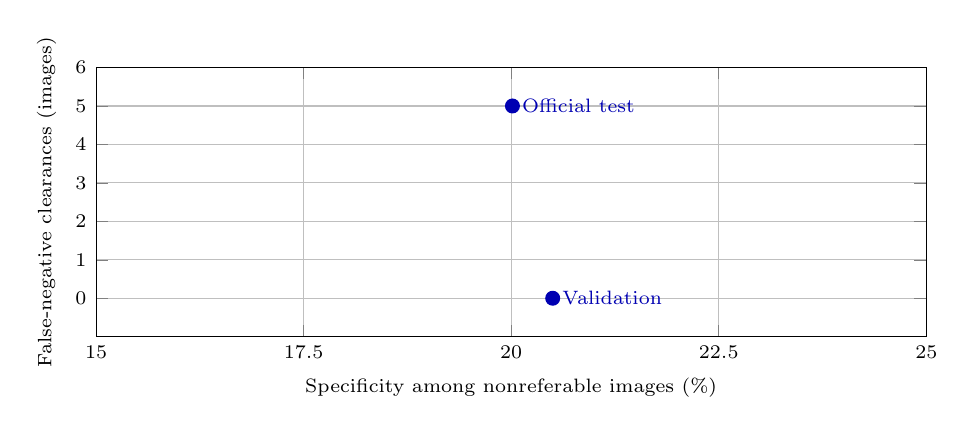
\begin{tikzpicture}
\begin{axis}[
    width=\columnwidth,height=5.0cm,
    xmin=15,xmax=25,ymin=-1,ymax=6,
    xlabel={Specificity among nonreferable images (\%)},
    ylabel={False-negative clearances (images)},
    xtick={15,17.5,20,22.5,25},ytick={0,1,2,3,4,5,6},
    grid=major,tick label style={font=\scriptsize},
    label style={font=\scriptsize},
    nodes near coords,nodes near coords style={font=\scriptsize,anchor=west},
    point meta=explicit symbolic]
\addplot[only marks,mark=*,mark size=2.5pt,blue!70!black] coordinates {
    (20.50,0) [Validation]
    (20.015,5) [Official test]
};
\end{axis}
\end{tikzpicture}
\caption{The frozen internal model-selection operating point did not retain zero observed misses on the official MMRDR-UWF test. Specificity remained low on both partitions. The test specificity interval is reported in Table~\ref{tab:official-test}; the two points are image-level summaries, not patient-level estimates.}
\label{fig:operating-transfer}
\end{figure}

The score ranking and selected operating point are distinct properties. Figure~\ref{fig:mmrdr-roc} makes their divergence visible: the test-derived image-level ROC curve is strong overall, while the frozen threshold operates at a high false-positive rate and has five observed misses. The alternative point attaining 100\% observed sensitivity is post-hoc because the test labels were inspected; it is shown only to describe the observed frontier, never as a candidate threshold.

\begin{figure}[t]
\centering
\begin{tikzpicture}
\begin{axis}[
    width=\columnwidth,height=5.2cm,
    xmin=0,xmax=1,ymin=0,ymax=1,
    xlabel={False-positive rate},ylabel={True-positive rate},
    xtick={0,0.2,0.4,0.6,0.8,1.0},ytick={0,0.2,0.4,0.6,0.8,1.0},
    grid=major,tick label style={font=\scriptsize},
    label style={font=\scriptsize},
    legend style={font=\tiny,at={(0.02,0.98)},anchor=north west},
]
\addplot[gray,dashed,no marks] coordinates {(0,0) (1,1)};
\addlegendentry{Chance}
\addplot[blue!75!black,thick,no marks] table[
    x=false_positive_rate,y=true_positive_rate,col sep=comma
] {reproducibility/mmrdr_roc_display_aggregate_20261019.csv};
\addlegendentry{Empirical ROC (AUC 0.9173)}
\addplot[only marks,mark=*,mark size=2pt,orange!85!black] coordinates {
    (0.799847,0.996118)
};
\addlegendentry{Frozen threshold}
\addplot[only marks,mark=square*,mark size=2pt,red!75!black] coordinates {
    (0.906035,1.0)
};
\addlegendentry{Post-hoc 100\% sensitivity}
\end{axis}
\end{tikzpicture}
\caption{Image-level empirical ROC curve from the already-inspected official MMRDR-UWF test scores (2,597 images). AUC uses all scores; the displayed curve samples the aggregate empirical envelope at 1\%-FPR increments. The frozen threshold gives 99.61\% sensitivity and 20.02\% specificity. The post-hoc 100\%-sensitivity point gives 9.40\% specificity and is descriptive only, not a candidate threshold. Patient-clustered uncertainty is unavailable.}
\label{fig:mmrdr-roc}
\end{figure}

All five false-negative clearances were grade 2, the lowest referable category; grades 3 and 4 were all referred. The 1,047 false referrals comprised 593 grade-0 and 454 grade-1 images. Table~\ref{tab:grade-errors} gives the complete grade-stratified action counts. This post-test descriptive decomposition localizes the observed errors at the grade-1/2 boundary, but it was not used to alter the evaluated model.

\begin{table}[t]
\centering
\caption{Official-test actions stratified by reference grade. Grade 0--1 are nonreferable; grade 2--4 are referable. This post-test descriptive analysis did not modify the model.}
\label{tab:grade-errors}
\begin{tabularx}{\columnwidth}{>{\centering\arraybackslash}p{0.10\columnwidth}rrr>{\raggedright\arraybackslash}X}
\toprule
Grade & Images & Referred & Cleared & Class-specific rate \\
\midrule
0 & 800 & 593 & 207 & 25.88\% specificity \\
1 & 509 & 454 & 55 & 10.81\% specificity \\
2 & 544 & 539 & 5 & 99.08\% sensitivity \\
3 & 358 & 358 & 0 & 100.00\% sensitivity \\
4 & 386 & 386 & 0 & 100.00\% sensitivity \\
\bottomrule
\end{tabularx}
\end{table}

This primary fixed-threshold result is the paper's raw-image test evaluation. It is not an untouched external-site cohort: training, validation, and test are partitions of MMRDR, and test scores were later inspected for explicitly post-hoc ranking and frontier diagnostics reported below. Those diagnostics were not used to alter the model, threshold, or preprocessing, but their existence means the test set is no longer untouched for future confirmatory analysis. The dataset paper describes the official UWF test partition as patient-level, but the released annotation table lacks patient identifiers, preventing independent verification or patient-clustered uncertainty analysis in this project.

\subsection{Frozen Replay}
The replay matches the frozen reference exactly: 270/385 true negatives (70.13\%), zero observed false-negative clearances among 463 gradable referable eyes, zero ungradable clearances among 133 ungradable cases, and 100\% binary action assignment. Source specificity ranged from 65.05\% on DDR and 66.93\% on DRTiD to 98.08\% on DeepDRiD. The pooled value is a case-weighted aggregate of these source-specific denominators and should not be interpreted as an estimate for a target clinic with a different source mix.

A patient-cluster bootstrap of the 385 negative eyes identified 364 negative-patient clusters: 206 in DDR, 31 in DeepDRiD (52 eyes), and 127 in DRTiD. The source-stratified 95\% percentile interval for replay specificity was 65.63--74.55\%; the eye-independent Wilson interval was 65.38--74.48\%. Their similarity indicates little interval change from clustering in this cohort, where 21 additional negative eyes belong to existing DeepDRiD patient clusters. Neither interval addresses the replay's zero observed misses. Because the operating policy and cohort were selected and inspected during development, the cluster interval is descriptive and conditional, not an uncertainty statement for new patients after selection.

The pooled replay is sensitive to dataset composition. The observed negative-eye weights were 53.51\% DDR, 13.51\% DeepDRiD, and 32.99\% DRTiD, yielding 70.13\% specificity. Giving each source equal weight yields 76.68\% (patient-cluster bootstrap 95\% percentile interval, 72.93--80.32\%). This 6.55-point difference is a reweighting of the same source-specific outcomes, not a model improvement. The patient-cluster bootstrap contrast for DeepDRiD minus DDR was 33.03 percentage points (95\% percentile interval, 25.24--40.29), and for DeepDRiD minus DRTiD was 31.15 points (22.05--40.16); the DDR-minus-DRTiD contrast was -1.88 points (-12.31--8.54). These are exploratory conditional contrasts. Source mix, case mix, score behavior, and dataset-specific selection are entangled, so the analysis cannot attribute the difference to camera, disease severity, or an intrinsic dataset property. Across all convex mixtures of the three observed source-specific rates, the arithmetic range is 65.05--98.08\%; this range is not a confidence interval. These results show why the pooled replay cannot be transported to an unspecified target population without a justified target source mixture.

DDR contributes 134 TN among 206 gradable negatives and 72 referrals; DeepDRiD contributes 51/52 TN with one referral; DRTiD contributes 85/127 TN and 42 referrals. The high pooled specificity is thus compatible with substantial source variation and a small high-specificity denominator. These differences may reflect case mix, camera domains, grading, and component channels; this audit does not establish that one dataset is intrinsically easier. Across the full cohort, 115/385 nonreferable records were referred, corresponding to the complement of specificity under the binary policy. This referral burden is relevant to deployment but is not a population false-positive rate estimate.

Table~\ref{tab:source-mixture} and Fig.~\ref{fig:source-mixture} report the source denominators and the two mixture summaries. The equal-source row is standardized from the same observed source rates; it is not a new cohort and must not be read as external validation.

\begin{table*}[t]
\centering
\caption{Observed source-specific replay outcomes and descriptive source-mixture summaries. Source intervals and contrasts are conditional patient-cluster bootstrap summaries of the exposed, selected cohort; they are not selection-adjusted or external-validation inferences.}
\label{tab:source-mixture}
\footnotesize
\setlength{\tabcolsep}{3pt}
\begin{tabularx}{\textwidth}{>{\raggedright\arraybackslash}p{0.18\textwidth}rrrrr}
\toprule
Source & \shortstack{Negative\\eyes} & \shortstack{Negative\\patients} & TN & \shortstack{Specificity\\(95\% cluster CI)} & \shortstack{Observed\\mixture weight} \\
\midrule
DDR & 206 & 206 & 134 & 65.05\% (58.25--71.36) & 53.51\% \\
DeepDRiD & 52 & 31 & 51 & 98.08\% (93.75--100.00) & 13.51\% \\
DRTiD & 127 & 127 & 85 & 66.93\% (58.27--74.80) & 32.99\% \\
\midrule
Observed pooled mixture & 385 & 364 & 270 & 70.13\% (65.63--74.55) & 100.00\% \\
\shortstack[l]{Equal-source\\standardization} & -- & -- & -- & 76.68\% (72.93--80.32) & 33.33\% each \\
\bottomrule
\end{tabularx}
\\[2pt]
\footnotesize All intervals are 50,000-replicate source-stratified patient-cluster percentile intervals, seed 20261019. The source-rate span 65.05--98.08\% is a descriptive mixture range, not an uncertainty interval. Equal-source weighting reuses the observed cases.
\end{table*}

\begin{table}[t]
\centering
\caption{Exploratory pairwise source contrasts in the exposed replay. Intervals are source-stratified patient-cluster bootstrap percentiles; not adjusted for policy selection, multiplicity, or cohort exposure.}
\label{tab:source-contrasts}
\footnotesize
\begin{tabularx}{\columnwidth}{>{\raggedright\arraybackslash}Xrr}
\toprule
Contrast & Difference (pp) & 95\% interval (pp) \\
\midrule
DeepDRiD $-$ DDR & 33.03 & 25.24--40.29 \\
DeepDRiD $-$ DRTiD & 31.15 & 22.05--40.16 \\
DDR $-$ DRTiD & $-1.88$ & $[-12.31,\,8.54]$ \\
\bottomrule
\end{tabularx}
\end{table}

\begin{figure}[t]
\centering
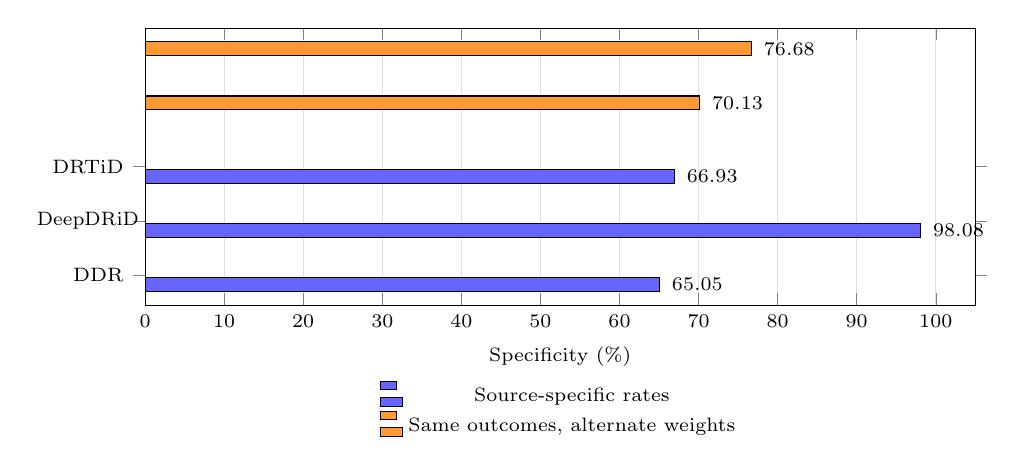
\begin{tikzpicture}
\begin{axis}[
    xbar,
    width=\columnwidth,
    height=5.1cm,
    xmin=0, xmax=105,
    xlabel={Specificity (\%)},
    symbolic y coords={DDR,DeepDRiD,DRTiD,Observed,Equal},
    ytick=data,
    yticklabels={DDR,DeepDRiD,DRTiD,Observed mix,Equal source},
    yticklabel style={font=\scriptsize,align=right,text width=1.1cm},
    xlabel style={font=\scriptsize},
    tick label style={font=\scriptsize},
    xmajorgrids=true,
    grid style={gray!25},
    nodes near coords,
    nodes near coords style={font=\scriptsize,anchor=west},
    every node near coord/.append style={xshift=1pt},
    bar width=5pt,
    enlarge y limits=0.14,
    legend style={font=\scriptsize,at={(0.5,-0.25)},anchor=north,legend columns=1,draw=none},
]
\addplot[fill=blue!60] coordinates {
    (65.05,DDR) (98.08,DeepDRiD) (66.93,DRTiD)
};
\addlegendentry{Source-specific rates}
\addplot[fill=orange!80] coordinates {
    (70.13,Observed) (76.68,Equal)
};
\addlegendentry{Same outcomes, alternate weights}
\end{axis}
\end{tikzpicture}
\caption{Observed replay specificity by source (blue) and two summaries of the same outcomes (orange). The observed mixture uses the cohort's negative-eye proportions; equal-source reweighting assigns one third to each source. The 6.55-point difference is compositional, not a model change, target-clinic estimate, or external validation.}
\label{fig:source-mixture}
\end{figure}

\subsection{Exposed ConvNeXt-Tiny Development Comparator}
The separate ConvNeXt-Tiny eye-bag model assigned an action to all 982 exposed development eyes. At its development-selected operating point it cleared 182/386 gradable nonreferable eyes (47.15\%), referred all 463 gradable referable eyes (0/463 observed misses), and referred all 133 known-ungradable cases. The source-specific true-negative counts were 112/207 for DDR, 27/52 for DeepDRiD, and 43/127 for DRTiD. Specificity was 169/274 (61.68\%) for grade 0 and 13/112 (11.61\%) for grade 1; grade-1 false referrals dominate the negative-case error burden. It referred 800/982 development eyes (81.47\%). Its test partition was not evaluated; this exposed development result is not compared with the MMRDR official-test result as a model ranking.

\subsection{Exploratory Post-Selection Accuracy Diagnostic}
On the 1,338 validation images, threshold cross-fitting yielded 1,126 correct classifications (84.16\% accuracy), comprising 660 true positives, 466 true negatives, 99 false positives, and 113 false negatives. Sensitivity was 85.38\%, specificity 82.48\%, and binary action assignment was 100\%. Fold thresholds were 1.266855, 1.266855, 1.220113, 1.266855, and 0.809623. This is a development-only accuracy diagnostic, not achievement of the project's clinical operating target: it misses 113/773 referable images, and its checkpoint was selected using all validation labels. Accuracy is reported descriptively because it was the threshold-selection objective; sensitivity, specificity, and the confusion counts are necessary to interpret it. Table~\ref{tab:accuracy-crossfit} summarizes these diagnostics. It is not an unbiased cross-validation estimate, test result, or evidence of autonomous clinical safety.

\begin{table}[t]
\centering
\caption{Exploratory post-selection accuracy diagnostic on three-source ResNet-50 validation scores; not the primary model result.}
\label{tab:accuracy-crossfit}
\small
\begin{tabularx}{\columnwidth}{>{\raggedright\arraybackslash}Xr}
\toprule
Metric & Result \\
\midrule
$N$ & 1,338 \\
Accuracy & 84.16\% \\
Sensitivity / specificity & 85.38\% / 82.48\% \\
TP / TN & 660 / 466 \\
FP / FN & 99 / 113 \\
Binary action assignment & 100\% \\
\bottomrule
\end{tabularx}
\\[2pt]
\footnotesize Validation-only, threshold-crossfit analysis; checkpoint epoch was selected on the full validation set. Not independent or unbiased confirmation.
\end{table}

Table~\ref{tab:replay-model-contrast} keeps this image-model result separate from the score-policy replay because both cohort membership and selection procedure differ.

\begin{table*}[t]
\centering
\caption{Selection-history evidence map for the principal analyses. The rows have different inputs and estimands and are not a head-to-head model comparison. The map records why an analysis is replay, internal development, a within-dataset evaluation, post-hoc diagnosis, or synthetic mechanism evidence.}
\label{tab:replay-model-contrast}
\footnotesize
\setlength{\tabcolsep}{3pt}
\begin{tabularx}{\textwidth}{>{\raggedright\arraybackslash}p{0.20\textwidth}>{\raggedright\arraybackslash}p{0.25\textwidth}>{\raggedright\arraybackslash}p{0.24\textwidth}X}
\toprule
Evidence object / input unit & Outcome-dependent selection history & Partition / identity status & Permissible inference \\
\midrule
Frozen ResNet-50 / raw UWF images, image unit & Head/checkpoint and threshold selected using internal image-level validation; threshold frozen before source-designated test scoring & Two positive test images have exact model-fit copies; patient IDs unavailable in local export & The primary fixed-threshold, image-level within-dataset outcome; not independent patient/site validation \\
Score-policy replay / precomputed component scores, eye unit & Source-specific ranks, weights, and cutoffs were developed using the same exposed score cohort later replayed & Same 981-eye cohort supplies policy references and reported outcomes & Deterministic implementation replay only; 70.13\% is not raw-image model performance \\
Grouped/nested procedures / precomputed scores, eye unit & Fold-level fits are separated within each run, but the cohort and component-family history predate the folds & Reuses the exposed 981-eye cohort; seeds reuse the same patients & Internal development and split-sensitivity evidence; not independent confirmation \\
Post-hoc MMRDR frontier / test logits, image unit & Alternative operating points were selected by searching inspected test scores against test labels & Same official test records used for the primary outcome; no patient IDs & Descriptive ranking/trade-off diagnostic only; no cutoff is eligible for model repair or deployment \\
ConvNeXt-Tiny / raw image bags, eye unit & Checkpoint and thresholds selected on the exposed validation subset; official test inference was skipped & Exposed 982-eye validation manifest; no test result & Development comparator only; no held-out performance claim \\
Controlled simulation / generated score channels, case unit & Candidate chosen on generated development data and evaluated on separately generated test data under a specified score model & Synthetic samples are independent by construction; no retinal records & Mechanism evidence under the stated generator only; not a retinal estimate or causal explanation \\
\bottomrule
\end{tabularx}
\end{table*}

The selection-history map in Table~\ref{tab:replay-model-contrast} is the organizing methodological output; the metric tables retain the counts needed to audit each result. The primary raw-image outcome is 99.61\% sensitivity (1,283/1,288), 20.02\% specificity (262/1,309; Wilson 95\% CI 17.94--22.27\%), 59.49\% accuracy, 59.81\% balanced accuracy, and 89.72\% referred (2,330/2,597), with five false-negative images. These are measured on the dataset's source-designated test partition, where a post-hoc byte audit found two positive test images with exact model-fit copies. The filtered analysis is descriptive, and neither result is independent clinical validation. The 70.13\% result is a transductive replay over stored scores, not the raw-image classifier's performance. The ConvNeXt result is exposed validation; neither secondary result is a head-to-head comparison with the primary test outcome.

To separate score ranking from the selected operating point, we computed threshold-free and threshold-varying diagnostics from the hash-verified frozen prediction export after the official test had already been inspected. Image-level ROC-AUC was 0.9173 and average precision was 0.9234. These are descriptive ranking summaries: the export does not contain usable patient identifiers, so patient-clustered uncertainty cannot be calculated. At the locked validation-selected threshold, sensitivity was 99.61\% and specificity 20.02\%. The retrospective test-label envelope reached 30.94\% specificity at at least 99\% sensitivity, 57.07\% at at least 95\%, and 74.41\% at at least 90\%; the best point with all 1,288 test positives referred had 9.40\% specificity. Every point on this envelope is selected by maximizing specificity under a sensitivity constraint on the same inspected test scores; it is therefore an optimistically selected descriptive bound, not a prespecified operating point. We report no inferential interval for this searched envelope: ordinary pointwise intervals would ignore both the within-test search and the unavailable patient clustering. These alternative cutoffs must not be used to select or repair the model. Thus, the observed limitation is not adequately described as a single threshold-transfer failure: even the test-derived envelope shows a substantial sensitivity--specificity trade-off on this partition. The grade-wise referral rates at the frozen threshold were 74.13\% for grade 0, 89.19\% for grade 1, 99.08\% for grade 2, and 100\% for grades 3 and 4, localizing most avoidable referral burden to nonreferable grades. Table~\ref{tab:mmrdr-posthoc-frontier} summarizes the diagnostic envelope; the script and aggregate output are listed in Table~\ref{tab:artifacts}.

\begin{table}[t]
\centering
\caption{Post-hoc sensitivity-constrained specificity envelope on the inspected MMRDR-UWF official test scores. These test-derived cutoffs are descriptive only and are not valid model-selection or deployment thresholds.}
\label{tab:mmrdr-posthoc-frontier}
\small
\begin{tabularx}{\columnwidth}{>{\raggedright\arraybackslash}Xrr}
\toprule
Sensitivity constraint & Observed sensitivity & Specificity \\
\midrule
100\% (zero observed misses) & 100.00\% & 9.40\% \\
$\geq$99\% & 99.07\% & 30.94\% \\
$\geq$98\% & 98.06\% & 41.33\% \\
$\geq$95\% & 95.03\% & 57.07\% \\
$\geq$90\% & 90.06\% & 74.41\% \\
$\geq$80\% & 80.05\% & 88.62\% \\
\bottomrule
\end{tabularx}
\end{table}

\subsection{Patient-Grouped Evaluation}
Table~\ref{tab:cv} summarizes pooled specificity and missed cases for the replay, patient-grouped procedures, and the post-hoc diagnostic.
\begin{table}[t]
\centering
\caption{Specificity and missed cases under alternative development procedures.}
\label{tab:cv}
\small
\setlength{\tabcolsep}{3pt}
\begin{tabularx}{\columnwidth}{>{\raggedright\arraybackslash}Xrrr>{\raggedright\arraybackslash}p{0.27\columnwidth}}
\toprule
Procedure & TN/385 & Sp. & Misses & Evidence class \\
\midrule
Same-cohort replay & 270 & 70.13\% & 0 & exposed \\
Fixed blend, 5-fold & 268 & 69.61\% & 3 & grouped development \\
Nested weights, 5$\times$4 & 248 & 64.42\% & 5 & nested development \\
Nested + margin & 253 & 65.71\% & 6 & nested development \\
Post-hoc margin & 243 & 63.12\% & 0 & held-out tuned \\
\bottomrule
\end{tabularx}
\end{table}

\subsection{Candidate-Set Sensitivity}
The initial seed shows 189/385 true negatives (49.09\%) and two misses for the label-screened panel versus 221/385 (57.40\%) and three misses for all aligned columns. Across five paired seeds, specificity averages 57.45\% (SD 4.79 points; range 49.09--60.78\%) for the shortlist and 56.31\% (SD 1.01; range 54.81--57.40\%) for all aligned columns. Mean misses are 2.6 and 4.2; neither panel achieves zero misses in any seed. The all-aligned panel is lower in four paired runs and higher in one; its mean paired contrast is -1.14 points (range -4.16 to +8.31). Applying the requested descriptive filter of fewer than five observed misses, the maximum among all ten panel-by-seed outcomes is 234/385 true negatives (60.78\%) with three misses, from the screened panel at seed 20261019. Because this is the maximum selected after observing repeated partitions, it is not a prespecified performance estimate. These are descriptive split-sensitivity values, not confidence intervals: repeated CV folds overlap, and seeds do not create new patients. Table~\ref{tab:candidatesensitivity} reports the five-seed summary; Fig.~\ref{fig:candidate-source} shows the initial-seed source breakdown, and Fig.~\ref{fig:panel-seed-sensitivity} shows the paired seed-specific estimates. The complete seed table is in the audit JSON.

\begin{table*}[t]
\centering
\caption{Five-seed candidate-panel sensitivity under the same five-outer/four-inner patient-grouped procedure. Means and ranges describe split sensitivity, not confidence intervals; each panel includes the established fused recipe. The cohort and artifact library were historically exposed.}
\label{tab:candidatesensitivity}
\footnotesize
\setlength{\tabcolsep}{3pt}
\begin{tabularx}{\textwidth}{>{\raggedright\arraybackslash}p{0.16\textwidth}>{\raggedright\arraybackslash}p{0.17\textwidth}>{\centering\arraybackslash}p{0.08\textwidth}>{\centering\arraybackslash}p{0.12\textwidth}>{\centering\arraybackslash}p{0.14\textwidth}>{\centering\arraybackslash}p{0.11\textwidth}>{\raggedright\arraybackslash}X}
\toprule
Candidate panel & Columns (DDR / DeepDRiD / DRTiD) & Mean TN / 385 & Mean specificity & Mean misses; zero-miss runs & Specificity range & Evidence class \\
\midrule
Oracle-contributor shortlist & 11 / 1 / 7 & 221.2 & 57.45\% & 2.6; 0/5 & 49.09--60.78\% & exposed dev. \\
All complete aligned columns & 44 / 40 / 119 & 216.8 & 56.31\% & 4.2; 0/5 & 54.81--57.40\% & exposed dev. \\
\bottomrule
\end{tabularx}
\end{table*}

\begin{figure}[t]
\centering
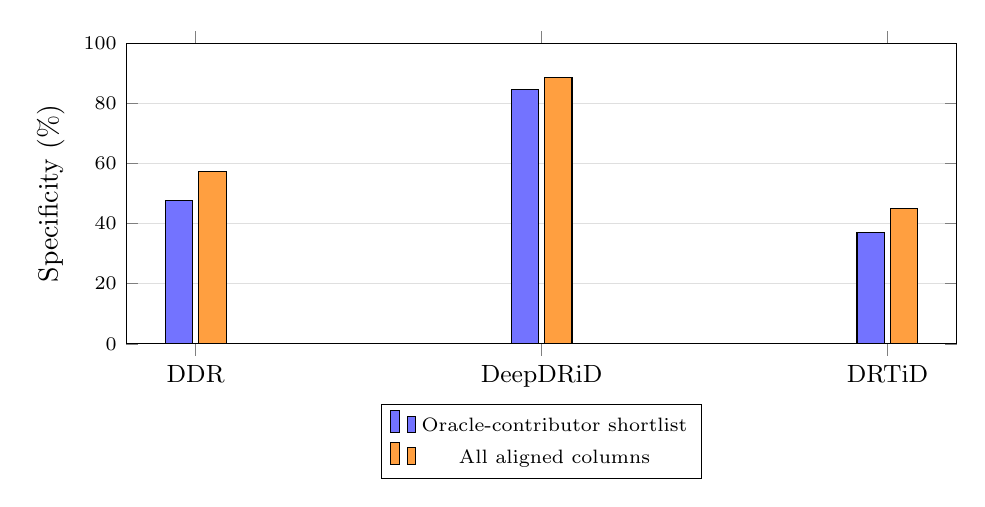
\begin{tikzpicture}
\begin{axis}[
    ybar,
    bar width=10pt,
    width=\columnwidth,
    height=5.4cm,
    ymin=0, ymax=100,
    ylabel={Specificity (\%)},
    symbolic x coords={DDR,DeepDRiD,DRTiD},
    xtick=data,
    x tick label style={font=\small},
    ymajorgrids=true,
    grid style={gray!25},
    legend style={font=\scriptsize,at={(0.5,-0.2)},anchor=north,legend columns=1},
    tick label style={font=\scriptsize},
]
\addplot[fill=blue!55] coordinates {(DDR,47.57) (DeepDRiD,84.62) (DRTiD,37.01)};
\addlegendentry{Oracle-contributor shortlist}
\addplot[fill=orange!75] coordinates {(DDR,57.28) (DeepDRiD,88.46) (DRTiD,44.88)};
\addlegendentry{All aligned columns}
\end{axis}
\end{tikzpicture}
\caption{Per-source specificity for the two nested panels. The corresponding miss counts (shortlist versus all aligned) are DDR 1/2, DeepDRiD 0/1, and DRTiD 1/0. These are development-fold outcomes on the exposed cohort, not external testing.}
\label{fig:candidate-source}
\end{figure}

\begin{figure}[t]
\centering
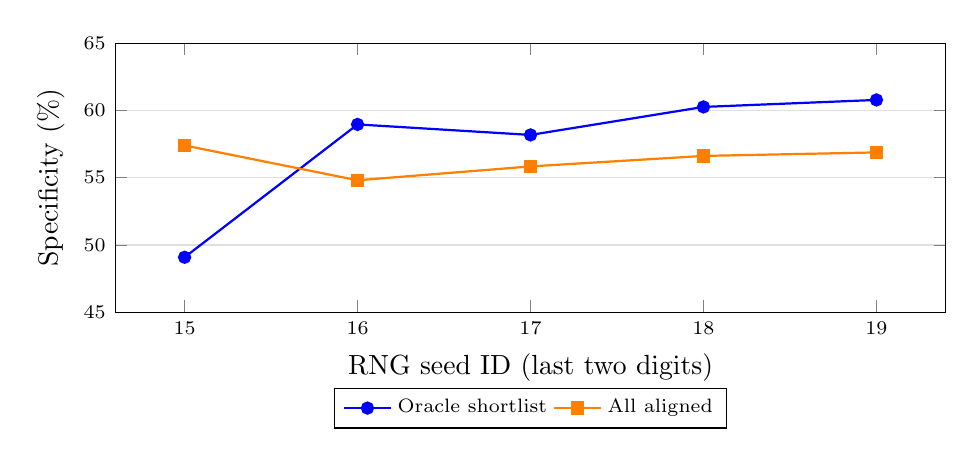
\begin{tikzpicture}
\begin{axis}[
    width=\columnwidth, height=5.0cm,
    ymin=45, ymax=65, ylabel={Specificity (\%)},
    symbolic x coords={seed15,seed16,seed17,seed18,seed19}, xtick=data,
    xticklabels={15,16,17,18,19}, xlabel={RNG seed ID (last two digits)},
    x tick label style={font=\scriptsize},
    ymajorgrids=true, grid style={gray!25},
    tick label style={font=\scriptsize},
    legend style={font=\scriptsize,at={(0.5,-0.28)},anchor=north,legend columns=2},
]
\addplot[mark=*,thick,blue] coordinates {(seed15,49.09) (seed16,58.96) (seed17,58.18) (seed18,60.26) (seed19,60.78)};
\addlegendentry{Oracle shortlist}
\addplot[mark=square*,thick,orange] coordinates {(seed15,57.40) (seed16,54.81) (seed17,55.84) (seed18,56.62) (seed19,56.88)};
\addlegendentry{All aligned}
\end{axis}
\end{tikzpicture}
\caption{Specificity across paired patient-fold RNG seeds (full IDs 20261015--20261019; integer identifiers, not dates). The first is the original split and the other four are added sensitivity splits. The contrast reverses after the initial seed. Points share one exposed cohort and are not independent replications or confidence intervals.}
\label{fig:panel-seed-sensitivity}
\end{figure}

This comparison isolates sensitivity to candidate-panel construction inside the coded nested analysis; it does not isolate all analyst degrees of freedom. Historical experiments that produced the artifact library were not nested anew, and a full-cohort oracle determined the shortlist. The finding is consequently a warning against reporting one selector result without documenting how its candidate universe was assembled.

\subsection{Controlled Zero-Miss Panel Simulation}
Figure~\ref{fig:panel-simulation} and Table~\ref{tab:panel-simulation} report the controlled simulation. Equation~\eqref{eq:single-channel-zero-miss} predicts a 16.67\% zero-miss frequency for the fixed-channel design ($n_d=60,n_t=300$); the observed $K=1$ frequencies are 18.10\% for $\rho=0$ and 15.60\% for $\rho=0.9$, with Monte Carlo intervals that include the reference. With independent candidate channels ($\rho=0$), searching 100 rather than one channel raised mean selected development specificity from 22.51\% to 55.45\%, while mean independent-test specificity rose from 22.48\% to 52.89\%; the fraction of replicates with zero test misses among 300 positives fell from 18.10\% to 0/2,000 (Monte Carlo Wilson 95\% interval, 0--0.19\%). At $\rho=0.9$, development specificity rose from 23.39\% to 41.64\%, while zero-miss frequency fell from 15.60\% to 1.20\% (Monte Carlo Wilson 95\% interval, 0.81--1.78\%). Under the perfect-correlation negative control ($\rho=1$), all panel sizes produced identical outputs and the observed zero-miss frequency was 17.40\% (Monte Carlo Wilson 95\% interval, 15.80--19.12\%), also consistent with the 16.67\% single-channel reference. These intervals quantify Monte Carlo error in estimating a simulation frequency, not uncertainty in retinal-cohort performance. The result demonstrates a specificity--miss tradeoff induced by selection under this specified synthetic model; it does not show that this mechanism caused the 70.13\% replay or empirical gaps.

\begin{figure}[t]
\centering
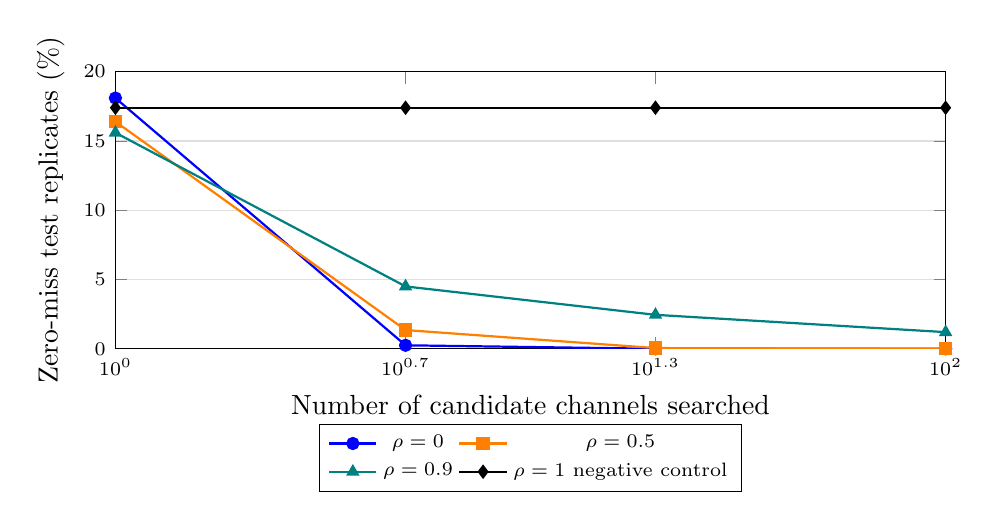
\begin{tikzpicture}
\begin{axis}[
    width=\columnwidth,height=5.1cm,
    xlabel={Number of candidate channels searched},
    ylabel={Zero-miss test replicates (\%)},
    xmin=1,xmax=100,ymin=0,ymax=20,
    xmode=log,log basis x=10,xtick={1,5,20,100},
    ytick={0,5,10,15,20},ymajorgrids=true,
    grid style={gray!25},tick label style={font=\scriptsize},
    legend style={font=\scriptsize,at={(0.5,-0.27)},anchor=north,legend columns=2},
]
\addplot[mark=*,thick,blue] coordinates {(1,18.10) (5,0.25) (20,0) (100,0)};
\addlegendentry{$\rho=0$}
\addplot[mark=square*,thick,orange] coordinates {(1,16.40) (5,1.35) (20,0.05) (100,0)};
\addlegendentry{$\rho=0.5$}
\addplot[mark=triangle*,thick,teal] coordinates {(1,15.60) (5,4.50) (20,2.45) (100,1.20)};
\addlegendentry{$\rho=0.9$}
\addplot[mark=diamond*,thick,black] coordinates {(1,17.40) (5,17.40) (20,17.40) (100,17.40)};
\addlegendentry{$\rho=1$ negative control}
\end{axis}
\end{tikzpicture}
\caption{Synthetic probability of zero misses on 300 independent positive cases after selecting the highest-development-specificity channel among $K$ equally discriminative channels. Each point is based on 2,000 Monte Carlo replicates. Candidate correlation attenuates the panel-size effect; perfectly identical channels yield no effect. This is a specified simulation, not clinical evidence.}
\label{fig:panel-simulation}
\end{figure}

\begin{table}[t]
\centering
\caption{Selected endpoint conditions from the controlled simulation. Intervals apply to Monte Carlo frequency only.}
\label{tab:panel-simulation}
\footnotesize
\setlength{\tabcolsep}{3pt}
\begin{tabular}{crrrrr}
\toprule
$\rho$ & $K$ & Dev. Sp. & Test Sp. & Zero-miss tests & MC Wilson 95\% CI \\
\midrule
0.0 & 1 & 22.51\% & 22.48\% & 18.10\% & 16.47--19.85\% \\
0.0 & 100 & 55.45\% & 52.89\% & 0.00\% & 0.00--0.19\% \\
0.9 & 1 & 23.39\% & 23.29\% & 15.60\% & 14.08--17.26\% \\
0.9 & 100 & 41.64\% & 40.37\% & 1.20\% & 0.81--1.78\% \\
1.0 & 1 & 22.42\% & 22.26\% & 17.40\% & 15.80--19.12\% \\
1.0 & 100 & 22.42\% & 22.26\% & 17.40\% & 15.80--19.12\% \\
\bottomrule
\end{tabular}
\end{table}

\subsection{Negative-sample sensitivity of candidate selection}
For the 100-channel panel, the paired sensitivity analysis separates development-set specificity optimism from zero-miss transfer frequency. At $\rho=0$, the development-minus-test specificity gap declined from 8.46 percentage points with 50 negatives to 0.57 points with 1,000, while independent-test specificity rose from 50.11\% to 53.78\%; zero test misses were observed in 0/2,000 replicates at all three sample sizes. The paired reduction in the gap between 50 and 1,000 negatives was 7.89 points (Monte Carlo normal 95\% interval, 7.60--8.19). At $\rho=0.9$, the gap declined from 4.04 to 0.25 points and independent-test specificity rose from 38.25\% to 40.08\%; zero-miss frequency changed only from 1.35\% to 1.10\%. The corresponding paired gap reduction was 3.79 points (3.50--4.08). These intervals quantify Monte Carlo uncertainty in a paired contrast under the specified generator, not sampling uncertainty for patients. Figure~\ref{fig:negative-sample-sensitivity} plots the simulated specificity-gap change and its Monte Carlo interval. Thus, within this synthetic model, increasing the negative sample used to rank candidates reduced estimated-specificity optimism; it did not remove the candidate-panel-associated zero-miss transfer pattern. The Wilson intervals and simulation-only scope are shown in Table~\ref{tab:negative-sample-sensitivity}. These findings are not estimates for retinal cases.

\begin{table*}[t]
\centering
\caption{Paired sensitivity of the 100-candidate synthetic selection result to the number of development negatives. Specificity gap is development minus independent-test specificity. Wilson intervals quantify Monte Carlo error for the simulated zero-miss frequency only.}
\label{tab:negative-sample-sensitivity}
\footnotesize
\begin{tabularx}{\textwidth}{c r r r r X}
\toprule
$\rho$ & $N^-_{\mathrm{dev}}$ & Dev. Sp. & Test Sp. & Gap (pp) & Zero-miss tests, \% (MC Wilson 95\% CI) \\
\midrule
0.0 & 50 & 58.57\% & 50.11\% & 8.46 & 0.00 (0.00--0.19) \\
0.0 & 200 & 55.37\% & 52.82\% & 2.55 & 0.00 (0.00--0.19) \\
0.0 & 1,000 & 54.34\% & 53.78\% & 0.57 & 0.00 (0.00--0.19) \\
0.9 & 50 & 42.29\% & 38.25\% & 4.04 & 1.35 (0.93--1.96) \\
0.9 & 200 & 40.79\% & 39.66\% & 1.13 & 1.20 (0.81--1.78) \\
0.9 & 1,000 & 40.33\% & 40.08\% & 0.25 & 1.10 (0.73--1.66) \\
\bottomrule
\end{tabularx}
\end{table*}

\begin{figure}[t]
\centering
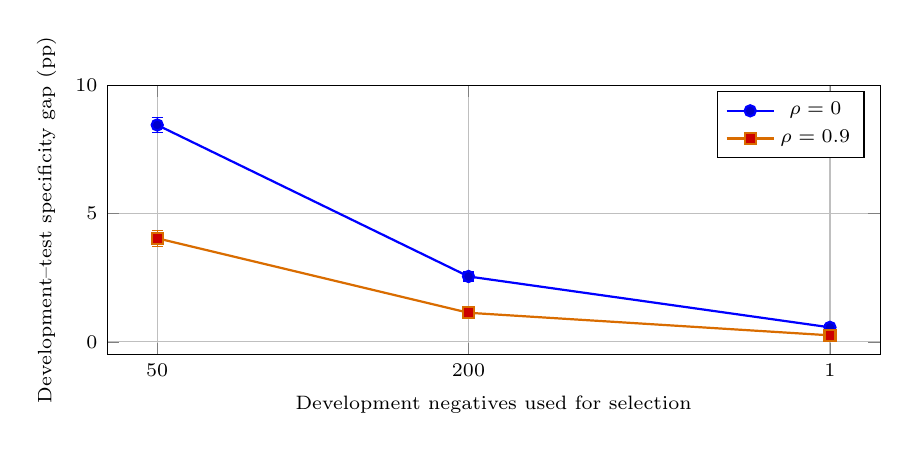
\begin{tikzpicture}
\begin{axis}[
    width=0.94\columnwidth,height=5.0cm,
    xmode=log,log basis x=10,xmin=40,xmax=1250,
    xtick={50,200,1000},xticklabels={50,200,1,000},
    xlabel={Development negatives used for selection},
    ylabel={Development--test specificity gap (pp)},
    ymin=-0.5,ymax=10,
    grid=major,tick label style={font=\scriptsize},
    label style={font=\scriptsize},
    legend style={font=\scriptsize,at={(0.98,0.98)},anchor=north east},
]
\addplot+[blue,mark=*,thick,error bars/.cd,y dir=both,y explicit]
coordinates {
    (50,8.4594) +- (0,0.29095)
    (200,2.55015) +- (0,0.17645)
    (1000,0.56565) +- (0,0.11862)
};
\addlegendentry{$\rho=0$}
\addplot+[orange!85!black,mark=square*,thick,error bars/.cd,y dir=both,y explicit]
coordinates {
    (50,4.0395) +- (0,0.30649)
    (200,1.1339) +- (0,0.17470)
    (1000,0.2540) +- (0,0.11416)
};
\addlegendentry{$\rho=0.9$}
\end{axis}
\end{tikzpicture}
\caption{Paired synthetic development-minus-test specificity gap for the 100-candidate selector as the number of development negatives increases. Whiskers are normal Monte Carlo 95\% intervals for each simulated mean gap, not patient-sampling intervals. All candidate channels have identical marginal quality under the generator; the result is mechanism-only and not a retinal performance estimate.}
\label{fig:negative-sample-sensitivity}
\end{figure}

The fixed-blend patient-grouped result differs from the replay by two true negatives and three misses. Nested weight/threshold selection yields 22 fewer true negatives than replay and five misses. The margin variant recovers five true negatives relative to nested selection, but its miss count rises to six. The post-hoc margin sweep recovers zero observed misses only after using held-out labels and at a lower specificity; it cannot be treated as a deployable operating point. In the original replay, 270 of 385 nonreferable cases are cleared and 115 are referred, while all 463 gradable referable and 133 ungradable records are referred. This describes the finite cohort; it does not establish zero population missed-disease risk.

The source-fold counts for fixed-recipe calibration are shown in Table~\ref{tab:fixedfold}. These counts reveal that an aggregate close to the replay does not imply fold-level stability. In particular, the single DeepDRiD false clearance occurs in a very small fold, while DDR and DRTiD each contribute a separate missed case. The fact that three errors occur in separate source domains suggests that a single pooled threshold adjustment would not be a complete diagnosis of the failure; the experiment uses source-specific calibration, yet still misses one positive in each source.

Table~\ref{tab:sourcegrouped} gives the source-level totals for the replay and fixed-recipe grouped estimate. The TN numerator is unchanged for DeepDRiD and DRTiD and decreases by two for DDR. The pooled specificity changes by only 0.52 percentage points, yet zero-miss status is lost. This is why a nearly identical specificity headline cannot stand in for joint reporting of the two endpoint dimensions.

\begin{table}[t]
\centering
\caption{Source-wise replay and fixed-recipe grouped results. Misses include referable or ungradable records assigned CLEAR.}
\label{tab:sourcegrouped}
\footnotesize
\setlength{\tabcolsep}{2pt}
\begin{tabular}{lrrrrr}
\toprule
Source & Neg. & \shortstack{Replay\\TN} & \shortstack{Replay\\miss} & \shortstack{Group\\TN} & \shortstack{Group\\miss} \\
\midrule
DDR & 206 & 134 & 0 & 132 & 1 \\
DeepDRiD & 52 & 51 & 0 & 51 & 1 \\
DRTiD & 127 & 85 & 0 & 85 & 1 \\
Pooled & 385 & 270 & 0 & 268 & 3 \\
\bottomrule
\end{tabular}
\end{table}

\begin{table*}[t]
\centering
\caption{Fixed-recipe patient-grouped out-of-fold results by source and fold. `Pos. miss' includes referable or ungradable cases cleared. Percentages are not reported because integer counts are more stable at these fold sizes.}
\label{tab:fixedfold}
\begin{tabular}{lrrrrr}
\toprule
Source & Fold & Held-out cases & Negatives & TN & Pos. misses \\
\midrule
DDR & 1 & 126 & 42 & 26 & 0 \\
DDR & 2 & 125 & 41 & 32 & 0 \\
DDR & 3 & 125 & 41 & 21 & 0 \\
DDR & 4 & 125 & 41 & 24 & 1 \\
DDR & 5 & 124 & 41 & 29 & 0 \\
DeepDRiD & 1 & 24 & 11 & 11 & 1 \\
DeepDRiD & 2 & 22 & 10 & 10 & 0 \\
DeepDRiD & 3 & 20 & 10 & 10 & 0 \\
DeepDRiD & 4 & 20 & 11 & 11 & 0 \\
DeepDRiD & 5 & 20 & 10 & 9 & 0 \\
DRTiD & 1 & 51 & 26 & 19 & 0 \\
DRTiD & 2 & 51 & 26 & 17 & 0 \\
DRTiD & 3 & 50 & 25 & 17 & 0 \\
DRTiD & 4 & 49 & 25 & 14 & 0 \\
DRTiD & 5 & 49 & 25 & 18 & 1 \\
\bottomrule
\end{tabular}
\end{table*}

For fixed-recipe cross-fitting, source totals are 132/206 TN for DDR, 51/52 for DeepDRiD, and 85/127 for DRTiD, totaling 268/385. Each source contributes one positive or ungradable miss. DDR fold specificity ranges from 51.22\% (21/41) to 78.05\% (32/41), with one miss in fold 4. DeepDRiD has four folds at 100\% and one at 90\% (9/10), with one miss in fold 1. DRTiD fold values range from 56.00\% (14/25) to 73.08\% (19/26), with one miss in fold 5. DeepDRiD's 10--11 negative cases per fold mean that a single eye shifts the fold percentage by roughly 9--10 points; integer counts are therefore more interpretable than isolated fold percentages.

\subsection{Expert-Selector Diagnostics}
The project tested whether complementary score channels could be turned into a selector. Candidate families included pairwise rank selection, nested regularized blends, single-expert routing, a nested OR rule, logistic and shallow-tree selectors, and a label-informed casewise oracle. All model-selection experiments draw on an already examined score library and cohort, so even patient-fold results are development diagnostics.

The pooled selector outcomes and the oracle's nondeployable, label-informed status are summarized in Table~\ref{tab:selectors}.

\begin{table*}[t]
\centering
\caption{Expert-routing diagnostics on the exposed 981-eye pool. The oracle is label-informed and cannot be implemented at inference.}
\label{tab:selectors}
\begin{tabular}{lrrrl}
\toprule
Procedure & TN/385 & Specificity & Misses & Interpretation \\
\midrule
Historical replay & 270 & 70.13\% & 0 & Exposed same-cohort reference \\
Pairwise rank selector, patient-fold & 245 & 63.64\% & 5 & Grouped development \\
Nested regularized blend & 216 & 56.10\% & 1 & Nested development \\
Nested single-expert route & 225 & 58.44\% & 2 & Nested development \\
Nested OR, internally shrunk & 206 & 53.51\% & 1 & Nested development \\
Nested nonlinear selector & 196 & 50.91\% & 1 & Nested development \\
Full-cohort casewise oracle union & 293 & 76.10\% & 0 & Uses each case's label \\
\bottomrule
\end{tabular}
\end{table*}

The oracle row asks whether at least one stored expert could clear each negative while maintaining the observed positive constraint. It chooses a favorable expert using the known label for that case, so the information is unavailable at inference. The 23-TN gap over the replay is a diagnostic upper description of score complementarity, not a reachable performance bound for a learnable selector. The failure of tested selectors to recover that margin suggests the stored channels did not produce a stable routing function with the available grouped data; it does not prove that all future selectors will fail.

A bounded one-score blend search tested 101 mixing weights from zero to one by source and recomputed its cutoff on the inspected labels. It reached 135/206 for DDR (from 134), 51/52 for DeepDRiD (unchanged), and 86/127 for DRTiD (from 85), or 272/385 (70.65\%). The two-eye same-cohort lift is rejected as progress because channel weights and cutoffs were selected from the evaluation labels. Repeating this grid would add no independent evidence.

\begin{figure}[t]
\centering
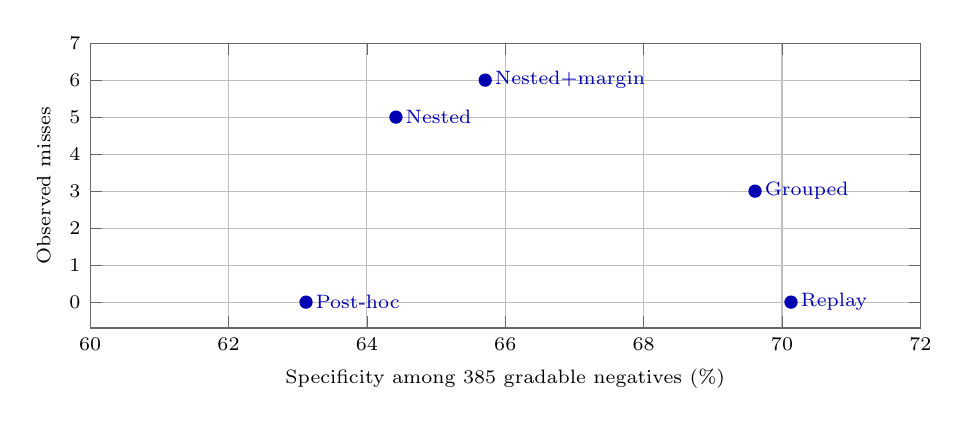
\begin{tikzpicture}
\begin{axis}[
    xmin=60, xmax=72,
    ymin=-0.7, ymax=7,
    width=\columnwidth, height=5.2cm,
    xlabel={Specificity among 385 gradable negatives (\%)},
    ylabel={Observed misses},
    xtick={60,62,64,66,68,70,72},
    ytick={0,1,2,3,4,5,6,7},
    grid=major,
    tick label style={font=\scriptsize},
    label style={font=\scriptsize},
    axis line style={black!60},
    tick style={black!60},
    nodes near coords,
    nodes near coords style={font=\scriptsize,anchor=west},
    point meta=explicit symbolic
]
\addplot[only marks,mark=*,mark size=2.2pt,blue!70!black] coordinates {
    (70.13,0) [Replay]
    (69.61,3) [Grouped]
    (64.42,5) [Nested]
    (65.71,6) [Nested+margin]
    (63.12,0) [Post-hoc]
};
\end{axis}
\end{tikzpicture}
\caption{Observed specificity--miss tradeoff for the five score-policy procedures in Table~\ref{tab:cv}. Misses include referable and ungradable clearances. The replay is selected on the same exposed cohort; the post-hoc zero-miss point uses held-out labels. Neither zero-miss point estimates performance on new patients.}
\label{fig:procedure}
\end{figure}

\begin{table}[t]
\centering
\caption{MMRDR-initialized fine-tuning on the audited 982-eye development validation manifest. All rows are development-only and thresholded on the same validation cohort.}
\label{tab:ft}
\begin{tabular}{lrrr}
\toprule
Epoch & TN/386 & Specificity & Observed misses \\
\midrule
Warm start (0) & 95 & 24.61\% & 0 \\
1 & 63 & 16.32\% & 0 \\
2 & 74 & 19.17\% & 0 \\
3 & 73 & 18.91\% & 0 \\
\bottomrule
\end{tabular}
\end{table}

Table~\ref{tab:ft} is not a clean epoch-selection comparison: the reference eyes were included in the validation manifest. It is included to show that training did not improve the selected zero-miss operating point in this run and to preserve the corrected split audit. Training loss reduction alone would not change that conclusion.

\subsection{Candidate-Transfer Diagnostic}
On the exposed reference cohort, the candidate alone has 54/385 true negatives (14.03\%) and two missed referable cases. The offline OR combination with the baseline has 273/385 true negatives (70.91\%), a 0.78-percentage-point descriptive increase, but also has two misses. It remains 16 true negatives below the 75\% arithmetic target and fails the zero-miss criterion. We do not promote it to a new frozen baseline.

The candidate was a high-resolution fine-tuned ResNet-50 transfer artifact rather than a mere threshold change. Its CLEAR decisions nevertheless overlapped strongly with the incumbent: the union gained only three TN, while introducing two positive misses. A small specificity increase is not a valid safety-constrained improvement when the positive constraint is violated. This is a negative result for this particular model, training path, and combination rule, not a conclusion about ResNet-50 or high-resolution retinal models generally.

\subsection{MMRDR-UWF Domain-Transfer Stress Test}
The best zero-miss point among the tested RETFound feature heads was 63/600 TN (10.50\%) for a logistic head; an RBF-SVM reached 60/600 (10.00\%). The internal ResNet+DINO / 448-pixel ResNet reference reached 202/600 (33.67\%) and AUROC 0.932. Adding 25\% of the RETFound-logistic rank produced 207/600 (34.50\%), five additional negatives, and AUROC 0.940. This comparison used the same internal model-selection labels for thresholding and candidate comparison; it is internal development estimation, not independent external testing, and does not revise the frozen 70.13\% reference.

Ranking metrics and high-sensitivity operating points need not move together. RETFound logistic features had AUROC 0.919 yet only 10.50\% specificity at the zero-miss cutoff on the internal model-selection subset. The internal reference had AUROC 0.932 and 33.67\% specificity; the fusion had AUROC 0.940 and 34.50\%. This descriptive pattern shows that high-tail ordering and threshold calibration matter in addition to global rank discrimination. Because labels were reused, it is not a clinical-utility result.

\subsection{MMRDR-Initialized Multi-Source Fine-Tuning}
On the 982-eye validation manifest, the MMRDR-initialized warm start reached 95/386 gradable negatives at zero observed misses (24.61\%). Fine-tuning at epochs 1, 2, and 3 yielded 63/386 (16.32\%), 74/386 (19.17\%), and 73/386 (18.91\%), respectively. A four-source balanced-sampling continuation selected the warm start; subsequent trained epochs remained below it. These results use a denominator of 386, not 385, because the audited validation manifest contains 982 eyes. Every historical reference eye was present among the validation rows, so model and threshold selection were exposed relative to the reference.

The original run summary incorrectly implied that the 981 reference eyes had been kept separate. A manifest audit corrected the record before this manuscript: 1,337 image rows across 982 eyes contained all 981 historical reference eyes in \texttt{source\_split=valid}. The corrected manifest therefore overlaps the full 981-eye reference; it is not an independent validation split. This correction supersedes the earlier separation statement and is retained in the audit trail as a provenance correction, not as new evidence of independence. The experiment did not produce an independent improvement over the 70.13 reference.

\subsection{Cross-Experiment Summary}
The procedure-level specificity contrast is visualized in Fig.~\ref{fig:procedure}; the separate raw-image model operating-point transfer is in Fig.~\ref{fig:operating-transfer}. No current model demonstrates the conjunction of high specificity, zero observed misses, and independent clinical validation. The frozen MMRDR classifier has the strongest evidence boundary because it was evaluated on the official held-out split, but it records five misses and only 20.02\% specificity. The 70.13\% replay and other zero-miss points use exposed or development-selected evidence. None supports autonomous clinical diagnosis \cite{openaiChatGPT}.

\section{Discussion}
The primary image-model finding is that ranking and screening operating-point performance diverged: image-level ROC-AUC was 0.9173, yet the frozen high-sensitivity rule produced only 20.02\% specificity and five false-negative images on the official test. The fixed threshold detected every referable image in validation but missed five on the official test. The test-derived envelope is even less favorable at zero observed misses, but it is post-hoc and cannot be used to repair or select the model. This exposes the practical cost of selecting a threshold to achieve zero observed validation misses. The result is not an argument that the architecture cannot improve; it shows that this frozen candidate, threshold, and training process did not achieve the desired sensitivity-specificity balance on the held-out split.

The broad operational issue is also visible in separate DR decision-policy work: Jena and Rayguru report 17.5\% specificity for their best single model at 95\% sensitivity on EyePACS, and lower referral burden for a weighted-ensemble strategy paired with a 90\% target \cite{jena2026}. This provides context for why sensitivity constraints and decision rules should be reported together; it does not validate the MMRDR result or show that one system is better. The datasets, label construction, models, sensitivity targets, and evaluation procedures differ, so no numerical cross-study ranking is warranted.

The 70.13\% value is separately a reproducible replay statistic, not an image-model estimate. Its reference vectors and thresholds were derived from the same cases that produce the headline, so exact replay checks implementation fidelity rather than generalization. Patient-grouped evaluation is more informative about within-cohort selection behavior, but previous global model-family search and cohort inspection mean those analyses remain development diagnostics.

The controlled simulation illustrates one possible selection mechanism without offering a causal explanation for the retinal findings. As the candidate menu grows, selection for specificity raises both the selected development and expected independent-test specificity in this construction, but it also raises the cutoff enough that the zero-miss constraint transfers less often. The correlation sweep indicates that effective candidate diversity matters: highly correlated candidates add less selection opportunity, and identical candidates add none. This supports recording the full candidate universe and selection history and reserving a cohort untouched by model-family and threshold decisions. It is not a new risk-control method and cannot convert exposed results into independent evidence.

The gap between the validation and official-test outcomes cautions against reporting a zero-miss result without documenting threshold selection and testing the frozen rule. This is particularly relevant to systems that maximize specificity subject to zero observed false negatives: the constraint itself can be repeatedly optimized against the development cohort. Future work should improve the classifier using development data, then evaluate a newly frozen candidate on an independently sourced, patient-disjoint cohort; the current official test must not be reused to tune it.

The source-specific findings also limit portability. DDR and DRTiD specificity are similar and substantially below the small DeepDRiD denominator. The pooled value is sensitive to the particular data mixture. Dataset-specific quantile mappings do not solve domain shift by themselves; they can encode the composition of the cohort used to form the ranks.

\subsection{What the 70.13\% Reference Does and Does Not Mean}
The number 70.13\% is useful as a frozen engineering reference: the deterministic scorer returns the same 270 TN, zero observed misses, and complete binary assignment when supplied the expected score rows. This verifies implementation consistency for the replay. It is not an estimate of what a new patient will experience, because the cases used to construct the rank references and thresholds are also the cases counted in the numerator and denominator. The exact arithmetic is real; its population interpretation is not established.

The source-mixture analysis sharpens this boundary: the observed dataset weights produce 70.13\%, whereas equal weighting of the same DDR, DeepDRiD, and DRTiD source-specific rates produces 76.68\%. This 6.55-point shift is purely compositional. Its exact arithmetic decomposition is $-13.12$ points from the lower DDR weight, $+19.45$ points from the higher DeepDRiD weight, and $+0.23$ points from the DRTiD weight change. The increase is driven by giving more weight to the small, high-specificity DeepDRiD subset; it does not improve the model, show that a balanced source mixture is clinically representative, or resolve the exposed-cohort selection problem. The source-cluster intervals and pairwise contrasts in Tables~\ref{tab:source-mixture} and~\ref{tab:source-contrasts} quantify resampling variability under the observed selected policy; the DeepDRiD contrasts are large in this sample, while DDR and DRTiD are not clearly separated by their interval. These comparisons do not isolate camera, grading, case-mix, or algorithm effects. The results demonstrate that the pooled headline depends on an arbitrary benchmark mixture and that future reporting should show source-specific denominators alongside any aggregate.

This distinction is not semantic hair-splitting. In a zero-miss search, a threshold is commonly set just below the least-risk positive. If that positive is selected after looking at all cases, the resulting cutoff has been optimized against the observed positive tail. Adding a model family, rank channel, source-specific margin, or post-processing rule expands the effective search even if only one final threshold is printed. An exact replay can reproduce a selected operating point perfectly while providing no independent evidence that the point will recur.

\subsection{Why Patient-Grouped Results Are Lower and Still Not Confirmatory}
The fixed grouped result preserves specificity close to the replay (69.61\% versus 70.13\%) but has three missed required eyes. We paired its held-out decisions to the deterministic replay for all 981 eye records. Among the 385 gradable nonreferable eyes, 268 decisions were CLEAR under both procedures, two changed from CLEAR to REFER, and no negative changed in the opposite direction; this gives 268/385 versus 270/385 and a paired difference of $-0.52$ percentage points. A source-stratified patient-cluster bootstrap over the 364 negative source--patient clusters gave a conditional percentile 95\% interval of $[-1.31,0.00]$ points. Among 596 referable or ungradable eye records, all three cross-fit missed-eye events were replay-REFER to cross-fit-CLEAR transitions; no such record was cleared by replay. The observed eye-level missed-required-eye rates were therefore 0/596 versus 3/596, a paired difference of $+0.50$ percentage points (conditional source-stratified patient-cluster bootstrap 95\% interval, $[0.00,1.17]$; 574 positive-or-ungradable source--patient clusters). Table~\ref{tab:paired-transitions} gives the complete paired transition counts. Thus, the near-equal negative clearance count masks a different safety outcome: the grouped procedure loses zero-miss status. Both intervals condition on the already inspected cohort and fixed paired decisions; they do not account for earlier candidate/model search or calibration/threshold selection and are not confirmatory performance intervals. The missed-eye interval includes zero and should not be read as evidence of a statistically resolved risk difference. The nested result is lower (64.42\%) with five missed required eyes, while the nested-margin result gains five TN and has six. These comparisons indicate sensitivity to how calibration and weight selection are conducted. They do not quantify an unbiased performance decrement from one universal deployment population: all source scores, the cohort, and the general candidate family had already been investigated.

\begin{table}[t]
\centering
\caption{Paired replay-to-cross-fit eye-action transitions on the exposed 981-eye cohort.}
\label{tab:paired-transitions}
\small
\begin{tabular}{lrrrr}
\toprule
Outcome subset & C/C & C/R & R/C & R/R \\
\midrule
Gradable nonreferable ($n=385$) & 268 & 2 & 0 & 115 \\
Referable or ungradable ($n=596$) & 0 & 0 & 3 & 593 \\
\bottomrule
\end{tabular}
\vspace{2pt}
\parbox{0.95\columnwidth}{\footnotesize C/C: CLEAR under both; C/R: replay CLEAR, grouped cross-fit REFER; R/C: replay REFER, grouped cross-fit CLEAR; R/R: REFER under both.}
\end{table}

Nested selection protects outer-fold labels from the local run's weight and threshold selection. It cannot retrospectively make all prior project decisions independent of those same patients. A new cohort with a frozen artifact remains necessary. If no external patient access is available, the scientifically valid action is to limit the claim to development analysis and prepare a prospective or independently sourced validation protocol, not to rename a development subset as ``test.''

\subsection{Zero-Miss Risk and the Difference Between a Count and a Guarantee}
For a fixed binary rule evaluated on $n$ independent positive patients with zero misses, the one-sided exact 95\% upper confidence bound for the miss probability is $1-0.05^{1/n}$. Requiring this bound to be at most 5\% yields $n\ge\log(0.05)/\log(0.95)$, or at least 59 positive patients with zero misses. This calculation assumes a prespecified rule and an appropriate independent sample; it does not apply as a certification statement to the repeatedly inspected pooled cohort or to selected thresholds. It also concerns positive-patient risk, not overall coverage, specificity, or performance on negative patients.

The audit's 463 positive eyes are not automatically 463 independent positive patients. The 981-eye pool contains 928 patients and at least one source has paired eyes. In addition, the model/threshold selection problem violates the fixed-rule condition. Therefore the large nominal positive-eye denominator cannot be substituted into a zero-miss certification formula to claim an upper risk bound. Certification must be planned at the patient level, with a frozen analysis and explicit treatment of both eyes from a patient.

\subsection{Interpretation of the MMRDR Model Findings}
The official held-out test confirms that the classifier does not meet a useful autonomous operating point: five of 1,288 referable images were cleared, while 1,047 of 1,309 nonreferable images were referred. The validation-to-test shift in observed misses is particularly important because the threshold was selected to include the least-risk validation positive. At the same time, the test provides one dataset-internal estimate for a fixed model, which is more informative than another retrospective threshold sweep. It does not tell us whether the errors arise from mislabeled borderline images, camera/quality variation, or model representation; patient-linked review and clinician adjudication are unavailable in the released export.

Earlier MMRDR development comparisons showed that a better AUROC did not ensure high specificity at a zero-miss cutoff on the internal model-selection subset. RETFound-head fusion and multi-source fine-tuning did not establish an improvement. The new official-test result should be interpreted as the evaluation of one frozen candidate, not as evidence that MMRDR, ResNet-50, or image classifiers generally are inadequate.

The MMRDR filename audit is equally important: independent numbering of CFP and UWF files prevents a join by numeric suffix from establishing eye correspondence. In multimodal retinal work, mistaken identity links can make an apparently paired cohort or paired loss invalid. The project corrected this before treating CFP as an auxiliary source. That correction should be retained in any successor publication and in data-preparation tests.

\subsection{Implications for Reproducible Model Development}
The experiments motivate a development protocol with explicit stage boundaries. First, define the target population, label boundary, unit of analysis, and action semantics. Second, create patient-disjoint development, calibration, and final evaluation partitions before candidate search. Third, log every model family and threshold decision made using development data. Fourth, freeze model weights, preprocessing, rank references, thresholds, and software versions before opening the final cohort. Finally, report both patient- and image-level counts, source-specific performance, failures, ungradable handling, and uncertainty. The final cohort should not be revisited for architecture or threshold repair.

For this project, a training-only partition can support model development; a development/validation partition can support model selection; a calibration partition can support a prespecified risk-control method; and an external certification cohort can support the final stated risk bound. These roles cannot be collapsed into one cohort by repeatedly resplitting after results are known. Public dataset availability is not equivalent to untouched status if the images have already influenced project decisions.

\subsection{Solo Authorship and Missing External Access}
The manuscript is explicitly written as a single-author research report. A lack of access to coauthors does not justify inventing collaborators, endorsements, clinical expertise, or institutional participation. It also does not prevent the author from preparing a full-length preprint or journal manuscript. It does, however, limit what can be claimed: no independent clinician reviewed the present result, no hospital supplied a prospective cohort, and no external group reproduced the analysis. Before any clinical journal submission, the author should seek qualified clinical/statistical review where possible, but the manuscript must remain accurate if that access is not obtained.

\subsection{Practical Research Contribution}
The image-model evaluation contribution is an explicit report of one frozen image classifier's development-to-official-test operating-point behavior, including the loss of zero-miss status and grade-stratified error pattern. The secondary project-specific contribution is a paired candidate-panel-by-split analysis of threshold selection. Across five seeds, the wider aligned panel does not improve the observed zero-miss point: no seed is zero-miss, mean specificity is 1.14 percentage points lower, and the paired effect changes sign across splits. The best observed result under the descriptive constraint of fewer than five misses is 60.78\% specificity with three misses, selected from ten panel-by-seed outcomes; it is not a prespecified or independent estimate. The initial favorable contrast therefore does not persist. Because the artifact library and cohort are historically exposed, this does not estimate population bias or establish a general effect of panel size. The model contribution is evaluation of an established classifier configuration, not architectural novelty or clinical validation.

\subsection{Implications for Product Claims}
The frozen ResNet-50 classifier is an actual raw-image model evaluated on a held-out official test partition, but it is not a clinically ready diagnostic product: it missed five referable images and referred almost nine of ten test images. Its evidence supports a bounded retrospective model-evaluation paper, not an autonomous-diagnosis claim. The 70.13\% score policy is a separate exposed score-level research artifact; it is not this classifier's performance. A 100\% action-assignment rate means the evaluator returned CLEAR or REFER for each test-manifest row, not that all real-world acquisitions are supported or safely diagnosed \cite{openaiChatGPT}.

\section{Limitations}
The MMRDR six-logit referable score includes index 5 although the experiment has no grade-5 categorical training examples. Binary referable, pairwise-ranking, and hard-boundary losses may indirectly supervise this logit through their aggregate score, but it receives no direct grade-5 categorical supervision. Since the checkpoint is unavailable, no ablation can establish whether this design choice materially affected performance; the direction and magnitude are unknown.
The primary model limitation is weak operating performance: at its frozen threshold it missed five referable images on the official test and referred 79.98\% of nonreferable images. The observed high sensitivity therefore comes with an impractically high false-referral burden and does not satisfy a zero-miss requirement. A separate combined-source ResNet-50 yields 84.16\% accuracy only in a post-selection threshold-crossfit diagnostic; its epoch was chosen using all development model-selection labels, and it misses 113 referable images. This value is not unbiased cross-validation or external confirmation. The source-designated UWF test is within the same dataset, not a second-site or prospective cohort; the exact-byte audit found two positive test images duplicated in model-fit data. Excluding those rows post hoc leaves the five misses and 20.02\% specificity unchanged, but does not remove the observed overlap or repair the test. The audit cannot detect near-duplicates or patient-level overlap. Local joins match all 2,597 prediction rows to the derived test manifest and source annotation CSV with grade/label agreement; however, the source CSV has no patient-link field and the derived manifest's patient and eye identifier columns are empty. Patient-clustered confidence intervals and independent verification of patient-level separation are therefore unavailable. The exact checkpoints are not included in the public checkout; the MMRDR checkpoint also omits full training arguments and feature-cache provenance, limiting clean-clone reproduction. The 70.13\% policy consumes precomputed scores rather than raw images. The separate ConvNeXt-Tiny result is development-selected, its test partition was not evaluated, and its checkpoint and eye-level predictions are absent from the public checkout. No prospective study, clinician workflow study, clinical risk certificate, calibration assessment, or regulatory assessment is reported.

Several further limitations constrain interpretation. First, eye-level pooling creates correlated observations when both eyes from one person are present; patient-grouped folds reduce this within procedure, but headline counts remain eye-weighted. The additional cluster bootstrap quantifies only sampling variability conditional on the selected frozen replay rule and cannot repair prior selection or historical cohort exposure. Second, source-specific training and label protocols are harmonized to a binary boundary for analysis; the paper does not provide a central re-adjudication of original images. Third, empirical rank transformations may be unstable when source sample sizes are small or when a new site has a different score distribution. Fourth, results can depend on image resizing, color normalization, encoder checkpoint, and quality pre-processing; incomplete checkpoint/preprocessing provenance blocks raw-image replication of the score policy.

Fifth, 100\% binary action assignment on the evaluated test rows does not count missing or unsupported deployment inputs, acquisition failures, or workflow failures. Sixth, the MMRDR internal model-selection carve-out is image-level because patient identifiers were not available. The dataset paper describes the official UWF test partition as patient-level, but that property could not be independently audited against the local export. Seventh, AUROC and zero-miss operating points from the candidate comparison do not imply a clinically acceptable threshold; the frozen model in fact made five test false negatives. Eighth, the later multi-source fine-tune is exposed relative to the historical reference due to audited overlap. Ninth, the analysis does not assess demographic subgroup performance, clinician adjudication, referral outcomes, acquisition repeatability, treatment benefit, cost-effectiveness, or workflow impact.

The related-work section is a focused narrative synthesis, not a systematic review. It is intended to situate the specific operating-point and selection-audit questions and does not claim exhaustive coverage of DR screening systems, multi-source learning, conformal risk control, or deployment studies. The manuscript's drafting and revision assistance is disclosed and cited in the sections identified in the acknowledgment \cite{openaiChatGPT}.

\section{Conclusion}
We evaluated a frozen ResNet-50 image classifier on the MMRDR-UWF official test partition at a threshold selected on development validation data. The observed zero-miss condition did not transfer: misses changed from 0/572 validation positives to 5/1,288 test positives. Sensitivity decreased by 0.39 percentage points and specificity by 0.48 points; specificity was already low on validation and remained low on test (20.50\% and 20.02\%). The classifier therefore fails the desired zero-miss/high-specificity operating point and is not ready for autonomous clinical diagnosis. This is evidence that an empirical zero-miss threshold on a finite development subset is not a guarantee, not evidence that specificity collapsed between partitions. Because the official test remains within MMRDR and the released rows lack patient identifiers, this result is not prospective or independently verified patient-level clinical validation.

The separate score-policy audit shows why headline replay values must not be conflated with raw-image model performance: its 70.13\% specificity is an exposed deterministic replay, the 84.16\% figure is a post-selection threshold diagnostic with substantial misses, and the frozen MMRDR classifier has a distinct held-out test result. A controlled simulation and an exact single-channel order-statistic reference further show why a development threshold with zero observed misses need not transfer, while making no claim that the synthetic mechanism explains the retinal outcomes. Together, the work provides a transparent model-evaluation and selection-audit case study, not a new architecture or clinical-performance claim. A future candidate must be improved using development data and evaluated on a new, independently sourced cohort under a locked protocol; this official test must not be revisited for repair.

The paired analysis adds an eye-level comparison of two procedures on the exposed score cohort: patient-grouped calibration retained a similar negative-clearance count (268/385 versus 270/385) but changed three referable or ungradable eye decisions from REFER to CLEAR (3/596 versus 0/596 observed missed required eyes; paired difference +0.50 percentage points, conditional 95\% patient-cluster interval 0.00--1.17). This shows why specificity alone is insufficient to compare operating policies and why the zero-miss replay cannot be treated as a transferable guarantee. The paired intervals are conditional on this selected cohort and fixed decisions; they do not repair exposure or establish future-patient performance \cite{openaiChatGPT}.

\section{Author and Contribution Statement}
Burak Ata Aksu is the sole human author, as confirmed by the author. The corresponding-author email supplied by the author is bataaksu1@gmail.com; no institutional affiliation or clinical site, medical school, or external evaluator is claimed. The analysis uses previously released datasets and derived project artifacts, subject to each source's terms. The author reports sponsor funding, but sponsor identities, award identifiers, and sponsor roles have not yet been supplied. The author intends to pursue pilot deployment of ActiveRetina; related organizational, ownership, or financial relationships require disclosure, and details remain pending. The study reports no new participant recruitment. The author reports that ethics approval was granted; the official approving institution or ethics committee, approval identifier, date and scope, and the disposition of informed consent for the source datasets have not yet been supplied. These details must be verified and documented before submission. The author confirms that aggregate research findings may be published; this is not a legal determination of dataset-license scope. Public ORCID and biographical details have not been supplied. The author is responsible for the final manuscript, scientific claims, and verification of all reported results.

\section{Claim-to-Evidence Ledger}
Table~\ref{tab:claims} makes the scope of each headline explicit. The labels \emph{deterministic replay}, \emph{internal development estimation}, and \emph{independent external testing} refer to distinct evidence classes and are not interchangeable. This ledger is intended to prevent descriptive replay or resampling results from being rewritten as clinical claims.

\begin{table*}[t]
\centering
\caption{Claim-to-evidence ledger. Deterministic replay denotes exact rerunning on the exposed reference records; internal development estimation denotes patient-grouped procedures on the previously inspected project cohort; independent external testing would require a frozen procedure evaluated on a new cohort not used for any project decision.}
\label{tab:claims}
\footnotesize
\setlength{\tabcolsep}{3pt}
\begin{tabularx}{\textwidth}{>{\raggedright\arraybackslash}p{0.24\textwidth}>{\raggedright\arraybackslash}p{0.29\textwidth}>{\raggedright\arraybackslash}X}
\toprule
Claim & Evidence in this study & \shortstack[l]{Status and permitted\\interpretation} \\
\midrule
The fixed score policy deterministically replays at 70.13\% specificity & 270/385 TN on 981 exposed reference records; source-stratified patient-cluster percentile interval 65.63--74.55\%, conditional on the selected policy and cohort & Verified implementation replay plus descriptive conditional interval; neither is independent validation or selection-adjusted inference \\
The frozen MMRDR classifier transfers its development-selected operating point to the official test & Official test: 1283/1288 TP, 5 FN, 262/1309 TN, 1047 FP; specificity 20.02\%; two positive test images have exact copies in model-fit data & Source-designated within-dataset test; not wholly image-disjoint, not patient-cluster audited, not prospective, and does not meet zero-miss/high-specificity goals \\
The ConvNeXt-Tiny comparator achieves 47.15\% specificity & 182/386 negatives cleared on an exposed validation manifest; test evaluation skipped & Internal development only; not comparable to the MMRDR official-test result \\
The multi-source ResNet-50 achieves 84.16\% pooled accuracy in the threshold-crossfit diagnostic & 1,126/1,338 rows; TP=660, TN=466, FP=99, FN=113 across DDR, DRTiD, and DeepDRiD & Post-selection diagnostic: epoch 6 was selected using all validation labels before threshold cross-fitting; not unbiased CV, independent validation, or clinical evidence \\
Candidate-panel search alters zero-miss transfer under the specified score model & 2,000-replicate Gaussian simulation; 100 independent channels: zero-miss frequency 0/2,000; identical-channel control matches the single-channel order-statistic reference & Synthetic mechanism evidence only; not a clinical estimate, causal explanation of the retinal results, or a new risk-control guarantee \\
The replay has zero observed referable/ungradable clearances & Zero in the same-cohort replay; these records informed policy selection & Descriptive replay count only; not a bound or guarantee on population risk \\
The evaluator assigns 100\% binary actions & Two-action rule emits CLEAR or REFER for supplied score rows & Score-row assignment only; not raw-image, workflow, or product coverage \\
Patient-grouped calibration preserves the replay's observed zero-miss status & On 596 referable or ungradable eye records, replay had 0 missed required eyes and grouped calibration had 3 (0.00\% vs. 0.50\%); paired difference +0.50 pp (conditional patient-cluster interval 0.00--1.17 pp) & Exposed-cohort internal comparison; interval includes zero and is conditional on fixed decisions; neither confirms patient-level population risk \\
Nested selection establishes a 75/0/100 operating point & Nested weights: 248/385 TN with five misses; nested margin: 253/385 with six & Not supported; neither procedure achieves the stated conjunction \\
MMRDR establishes independent external-site performance & One official held-out partition within MMRDR; no other site or dataset & Not supported; no independent site, prospective cohort, or external dataset \\
The system is ready for autonomous diagnosis & Frozen model missed five official-test referable images and specificity was 20.02\% & Not supported; not clinically ready \\
\bottomrule
\end{tabularx}
\end{table*}

\appendices
\section{Replay Specification}
The reference policy can be reproduced only when the correct source label and three component values are provided for each row. The implementation first maps values to source-specific midranks, applies the source's fixed weighted sum, applies the threshold and the DDR quality override, and emits one action. The essential stored operating-point constants are: DDR component weights $(0.50,0.10,0.40)$, threshold 0.22224, and quality override threshold 0.0018599; DeepDRiD weights $(0.20,0.40,0.40)$ and threshold 0.435849; DRTiD weights $(0.72,0.08,0.20)$ and threshold 0.34496. The exact score channel names are given in Section III-B. Values are included for deterministic replay, not recommended as new-site thresholds.

For each data row, the evaluator must retain the source, eye identifier, patient identifier where available, binary grade/gradability label, component values, reference-rank values, final score, threshold, override state, and action. A minimal audit should verify: each image appears once per intended eye view; patient groups do not cross folds; score channels are finite; all weights sum to one; threshold comparisons use the documented inclusive inequality; ungradable rows cannot be cleared; and summary counts equal a direct confusion-count reconstruction. The current source artifact verifies aggregate replay equality. A journal supplement should additionally provide a per-record output hash or a reproducible prediction file when dataset licenses permit.

\section{Selection Protocol and Leakage Audit}
The development chronology is relevant to the meaning of the reported estimates. First, component models and score outputs were generated for the public-source cohort. The pooled scores and labels were inspected during candidate development. Source-specific rank references and thresholds were then selected to maximize specificity subject to zero observed misses on this pool. The same data subsequently served as the named 70.13 reference. Later patient-grouped experiments re-fit calibration and, in nested variants, weights and thresholds within folds. However, the global component family, channels, cohort, and research question had already been informed by the full pool.

The evidence hierarchy is: deterministic replay is an implementation check; grouped and nested score-policy procedures are internal development estimates; the MMRDR-UWF official test is a frozen evaluation on the source-designated test partition, with two byte-identical test images also present in model-fit data; post-hoc margins, duplicate-exclusion counts, and oracle rows are descriptive diagnostics. No result is a prospective or independent-site clinical validation estimate. If a later independent cohort is acquired, freeze the artifact and analysis plan before outcomes are inspected and do not use that cohort for repair after its result.

The MMRDR audit has distinct split boundaries. The local UWF validation split has no exported patient IDs and is image-level; it was used for thresholding and candidate comparison. The source annotation CSV contains image-level annotations and laterality but no patient-link field. The official test manifest contains patient/eye ID columns but no nonempty values, and its prediction export has no such columns; exact image-ID joins to the predictions and source annotations verify row membership and labels only, not grouping. An exact-byte audit found two official-test images with copies in internal model-fit data; this post-hoc procedure cannot rule out near-duplicates or patient-level overlap. The later multi-source fine-tune's validation manifest included all 981 historical reference eyes, as established by direct ID intersection, so it is not an independent holdout. The cached-head ResNet-50 evaluation on the official MMRDR-UWF test partition is not wholly image-disjoint from fitting and must not be described as independent confirmation or reused for successor evaluation. The official test and exposed 981-eye replay are not concatenated into a synthetic cohort.

\section{Proposed Independent Evaluation Protocol}
A confirmatory study should specify the clinical use and target population first, then create a patient-level cohort whose members do not appear in training, model selection, score-reference construction, threshold selection, or prior exploratory analysis. The frozen package should include: (1) architecture and checkpoint hashes; (2) input file and color-space contract; (3) resizing and normalization; (4) quality/gradability policy; (5) every component output definition; (6) source or site mapping rules; (7) score reference vectors and fusion constants; (8) threshold and equality semantics; (9) software environment and deterministic inference settings; and (10) the statistical analysis plan.

The evaluation unit for a screening claim should be predeclared as patient, eye, or encounter. If both eyes are analyzed, uncertainty must account for within-patient correlation, and both eyes should remain in the same partition. The reference standard should be independent of the model output and should specify adjudication for borderline grades and ungradable images. The primary endpoint should state whether a miss means referable disease, ungradable disease, or both; secondary endpoints should include specificity, sensitivity, referral fraction, gradability, subgroup counts, and calibration if a probability is emitted.

For a zero-miss target, the policy must be frozen before certification. If no positive patient is missed among $n$ independent representative positive patients, the one-sided 95\% exact upper limit is $1-0.05^{1/n}$. At least 59 zero-miss positive patients are needed for this bound to fall at or below 5\%. This sample-size statement is conditional on the candidate being fixed and the cohort being appropriate; it does not guarantee specificity or coverage. If the method fails, the cohort becomes development data and a new untouched certification cohort is required for a later candidate.

\subsection{Prespecified Analysis Sequence}
For clarity, a future confirmatory run can be specified as the following ordered analysis. (1) A data custodian prepares the patient-level manifest and confirms that no participant appears in training, calibration, threshold selection, or earlier exploratory analysis. (2) The model owner deposits the frozen artifact hash and input contract before receiving labels. (3) A runner executes deterministic inference on all eligible images and logs decode, preprocessing, and model failures without manually dropping difficult records. (4) The reference standard is joined only after predictions are sealed. (5) The primary table reports patient-level positive outcomes, eye-level specificity with patient-clustered uncertainty, ungradable handling, image failures, and source-specific metrics. (6) The signed result package records the code revision, artifacts, manifest hash, analysis timestamp, and any deviations. The current study has no independent custodian or site, so this is a proposed protocol, not a process already completed.

The primary estimand must also be explicit. For patient-level screening, define a patient-positive as having referable disease in either eye, and count the patient as missed if the system clears both eyes or otherwise fails the predefined referral rule. For eye-level specificity, each gradable nonreferable eye is an eligible negative, but confidence intervals should cluster by patient. If the product's action is issued per encounter rather than per eye, the encounter-level aggregation rule must be prespecified. Reporting all three units as if they were interchangeable would overstate the amount of independent information.

\subsection{What the Current Cohort Can Support}
The present analysis supports descriptive replay and grouped-selection audits plus one frozen raw-image classifier evaluation on the MMRDR-UWF official test. It cannot identify performance at unseen clinics; demonstrate a calibration or risk guarantee; compare clinical outcomes; establish a clinically validated threshold; measure generalization to a camera/site outside the reported study; or support a claim that every raw image can be diagnosed safely. The test result itself is unfavorable for intended autonomous use, with five misses and 20.02\% specificity.

The next scientifically valid model study is to use training/development data only to improve the frozen classifier, lock preprocessing, weights, threshold, and evaluation code, then test once on a newly sourced patient-level cohort with exportable patient identifiers and an appropriate reference standard. The existing MMRDR official test has now been used and cannot be reused to claim confirmation for a successor. If a cohort suitable for risk certification is unavailable, report uncertainty honestly and retain clinician review; a point metric alone cannot substitute for the predeclared evidence criterion.

\section{Artifact and Reproduction Map}
The principal repository artifacts associated with this manuscript are listed in Table~\ref{tab:artifacts}. Paths are repository-relative and identify evidence already present in the project checkout; they do not imply that public images or every component checkpoint are redistributed.

\begin{table*}[t]
\centering
\caption{Artifact map and role in the analysis.}
\label{tab:artifacts}
\footnotesize
\setlength{\tabcolsep}{3pt}
\begin{tabularx}{\textwidth}{>{\raggedright\arraybackslash}p{0.43\textwidth}>{\raggedright\arraybackslash}X}
\toprule
Artifact & Role and evidence boundary \\
\midrule
\path{src/active_retina/exposed_expert_policy.py} & Deterministic score-policy evaluator; consumes component scores, not raw images \\
\path{results/deployable_exposed_baseline_7013_20261013_with_components/summary.json} & Frozen replay counts and explicit exposed-artifact status \\
\path{results/crossfit_expert_calibration_20261013_corrected/summary.json} & Fixed-recipe patient-grouped calibration results \\
\path{results/nested_crossfit_expert_weights_20261013/summary.json} & Five outer/four inner fold selection summary \\
\path{results/nested_crossfit_expert_weights_margin_20261013/summary.json} & Nested safety-margin diagnostic \\
\path{results/posthoc_zero_miss_margin_sweep_20261013.json} & Held-out-label post-hoc frontier; not a selected model \\
\path{paper/reproducibility/zero_miss_panel_simulation.py} & Controlled synthetic mechanism simulation; not clinical evidence \\
\path{paper/reproducibility/zero_miss_panel_simulation_results.json} & Aggregate Monte Carlo output (seed 20261016; 2,000 replicates per condition) \\
\path{paper/reproducibility/paired_replay_crossfit_audit.py} & Paired replay-versus-grouped action audit; requires local row-level score inputs \\
\path{paper/reproducibility/paired_replay_crossfit_audit_20261020.json} & Identifier-free aggregate transitions, paired bootstrap interval, and input hashes; not independent validation \\
\path{models/mmrdr_uwf_resnet50_cached_head_candidate_20261013.pt} & ResNet-50 plus trained linear head; historical SHA-256 begins \texttt{23578889}, but checkpoint bytes are absent from the current checkout and the digest is not reverified \\
\path{results/mmrdr_uwf_official_test_20261013.csv} & Local official UWF test manifest; SHA-256 begins \texttt{42f5cf01}; contains restricted dataset-derived rows \\
\path{src/active_retina/evaluate_mmrdr_candidate.py} & One-shot frozen test evaluator with checkpoint marker and exact operating-point metrics \\
\path{paper/reproducibility/mmrdr_uwf_official_test_run_card.json} & Machine-readable artifact/output hashes, frozen metrics, and explicit provenance gaps; does not include the checkpoint or test rows \\
\path{results/mmrdr_uwf_cached_head_20261013/summary.json} & Retained ResNet-50 UWF development-candidate aggregate used in Table~\ref{tab:mmrdr} \\
\path{results/mmrdr_uwf_dino_head_dev_20261013/summary.json} & Retained DINO UWF development-candidate aggregate used in Table~\ref{tab:mmrdr} \\
\path{results/mmrdr_uwf_dino_hardhead_dev_20261013/summary.json} & Retained DINO hard-head development-candidate aggregate used in Table~\ref{tab:mmrdr} \\
\path{results/mmrdr_embedding_heads_20261013/summary.json} & ResNet/DINO feature-head development aggregates used in Table~\ref{tab:mmrdr} \\
\path{results/mmrdr_uwf_retfound_eyepacs_heads_20261013/summary.json} & RETFound-EyePACS head development aggregates used in Table~\ref{tab:mmrdr} \\
\path{results/mmrdr_retfound_fusion_20261013/summary.json} & Same-validation rank-fusion diagnostics used in Table~\ref{tab:mmrdr} \\
\path{results/expert_selector_nested_crossfit_20261012.json} & Patient-fold pairwise-rank selector aggregate in Table~\ref{tab:selectors} \\
\path{results/expert_selector_nested_crossfit_oof_threshold_20261012.json} & Nested blend, single-expert, and OR selector aggregates in Table~\ref{tab:selectors} \\
\path{results/expert_selector_nested_crossfit_nonlinear_20261012.json} & Nested nonlinear-selector aggregate in Table~\ref{tab:selectors} \\
\path{results/expert_score_oracle_union_20261012.json} & Label-informed, nondeployable oracle aggregate in Table~\ref{tab:selectors} \\
\path{results/combined_mmrdr_qualitygate_balanced_allft_20261013/summary.json} & Four-epoch development history used in Table~\ref{tab:ft}; validation rows overlap the exposed reference cohort \\
\path{paper/submission/mmrdr_validation_epoch_trace_2026-10-16.csv} & Aggregate 26-epoch validation-selection trace; repeated use of one validation cohort, not independent evidence \\
\path{paper/reproducibility/export_mmrdr_validation_trace.py} & Rebuilds the trace from the tracked summary and checks count arithmetic and recorded zero-miss selection \\
\path{results/mmrdr_uwf_cached_head_20261013/summary.json} & Tracked aggregate epoch history used to derive the validation trace; contains no image-level predictions \\
\path{results/mmrdr_uwf_resnet50_official_test_20261015/summary.json} & Actual frozen official-test counts, uncertainty, and evidence boundary \\
\path{src/active_retina/analyze_mmrdr_test_frontier.py} & Hash-checked, post-hoc threshold-free ranking and sensitivity-constrained test-score diagnostics; does not select a threshold \\
\path{paper/reproducibility/mmrdr_test_score_diagnostic_20261019.json} & Aggregate ROC-AUC, average precision, grade-wise referral rates, and retrospective test-label frontier \\
\path{paper/reproducibility/mmrdr_roc_display_aggregate_20261019.csv} & Aggregate-only ROC display grid used in Fig.~\ref{fig:mmrdr-roc}; no per-image records \\
\path{paper/reproducibility/audit_mmrdr_exact_duplicate_impact.py} & SHA-256 audit of original image bytes across source partitions and model-fit split; aggregate-only output \\
\path{paper/reproducibility/mmrdr_exact_duplicate_impact_20261019.json} & Post-hoc overlap sensitivity result: two positive official-test rows duplicated in model-fit data; exclusion leaves five misses and specificity unchanged \\
\path{docs/mmrdr_transfer_and_retfound_development_20261013.md} & MMRDR provenance, domain-transfer results, and official-test boundary \\
\path{docs/70_13_to_75_candidate_20261013.md} & Fine-tune split correction and balanced-sampling results \\
\path{docs/expert_selector_nested_crossfit_20261012.md} & Expert selector experiments, oracle caveat, and source patient accounting \\
\bottomrule
\end{tabularx}
\end{table*}

The MMRDR-UWF run card and aggregate result (Table~\ref{tab:artifacts}) record the frozen validation threshold, official-test counts, specificity interval, image-row missed-risk bound, and non-certification status. The recorded checkpoint and manifest digests are historical provenance only: their bytes are absent from the public checkout, so the digests cannot be reverified there. Although the trainer, extractor, development manifest, and feature-cache hashes were recovered, the actual launch arguments, checkpoint bytes, feature cache, source-model weight revision, and full run environment are unavailable for clean reproduction. The official-test summary is an evaluation output, not a license to redistribute source rows or images. The older 70.13\% score-policy replay is also not regenerated by the clean-clone audit because its per-eye score/label rows remain local pending confirmation of redistribution permission. These reproducibility and rights boundaries are recorded in the run card and submission checklist; no raw images are included.

\section{Outer-Fold Selection Record}
The nested analysis is easier to audit when the outer predictions are presented source by source. Table~\ref{tab:nestedfold} transcribes the fold-level values from the saved run summary. The selected weights vary materially between folds, particularly in DeepDRiD and DRTiD. This variation is not by itself proof of instability because folds are finite and channel scales are empirical; together with the misses and modest denominators, it does show that the nested procedure does not settle on one evidently invariant source-specific recipe.

\begin{table*}[t]
\centering
\caption{Nested five-outer/four-inner-fold selection record. Weight columns correspond to the three ordered score channels for each dataset as defined in the frozen policy section. Thresholds and fold outcomes are development diagnostics; every patient fold was previously exposed to project-level research.}
\label{tab:nestedfold}
\footnotesize
\setlength{\tabcolsep}{3pt}
\begin{tabular}{llrrrrrl}
\toprule
Source & Fold & \shortstack{Held-out\\patients} & Negatives & TN & Misses & \shortstack{Selected\\weights} & Threshold \\
\midrule
DDR & 1 & 126 & 42 & 26 & 0 & (0.5, 0.0, 0.5) & 0.22445 \\
DDR & 2 & 125 & 41 & 32 & 1 & (0.6, 0.3, 0.1) & 0.21220 \\
DDR & 3 & 125 & 41 & 21 & 0 & (0.5, 0.0, 0.5) & 0.22900 \\
DDR & 4 & 125 & 41 & 22 & 0 & (0.8, 0.0, 0.2) & 0.22000 \\
DDR & 5 & 124 & 41 & 28 & 1 & (0.3, 0.4, 0.3) & 0.21397 \\
DeepDRiD & 1 & 12 & 11 & 10 & 0 & (0.3, 0.6, 0.1) & 0.43659 \\
DeepDRiD & 2 & 11 & 10 & 10 & 0 & (0.0, 0.4, 0.6) & 0.43810 \\
DeepDRiD & 3 & 10 & 10 & 6 & 0 & (0.2, 0.2, 0.6) & 0.42791 \\
DeepDRiD & 4 & 10 & 11 & 10 & 0 & (0.2, 0.5, 0.3) & 0.45116 \\
DeepDRiD & 5 & 10 & 10 & 3 & 1 & (0.5, 0.1, 0.4) & 0.39419 \\
DRTiD & 1 & 51 & 26 & 19 & 0 & (0.9, 0.1, 0.0) & 0.33970 \\
DRTiD & 2 & 51 & 26 & 17 & 0 & (0.5, 0.0, 0.5) & 0.32161 \\
DRTiD & 3 & 50 & 25 & 13 & 0 & (0.0, 0.2, 0.8) & 0.31800 \\
DRTiD & 4 & 49 & 25 & 13 & 0 & (0.7, 0.1, 0.2) & 0.34876 \\
DRTiD & 5 & 49 & 25 & 18 & 2 & (0.7, 0.0, 0.3) & 0.34527 \\
\bottomrule
\end{tabular}
\end{table*}

The outer-fold table has an important reading rule. A threshold in one fold is defined on that fold's training/calibration scores and does not share an absolute probability meaning with a threshold from another fold. Scores have already passed through source-specific empirical ranks, and each fold has its own reference data. The threshold values are included for reproducibility, not as an average cutoff to deploy. The small DeepDRiD folds make both weights and thresholds particularly sensitive to individual patient records.

The nested-margin version reuses the same outer partition but selects a nonnegative safety margin in the inner folds. Across its 15 source-fold units, the margins range from zero to 0.03 for DDR and DeepDRiD, and 0.005 to 0.02 for DRTiD. It returns six misses overall. These selected margins do not constitute a portable safety factor: they are score-space adjustments on fold-specific empirical ranks and do not translate into a fixed clinical risk reduction.

\section*{Reproducibility and Data Availability}
The artifact map in Table~\ref{tab:artifacts} identifies the policy evaluator, aggregate summaries, run card, paired replay-versus-grouped audit, and simulation materials. The tracked paired-audit receipt records 981 paired decisions and a conditional source-stratified patient-cluster bootstrap interval for the fixed decision difference; its script requires the local row-level score/label input and patient manifest, neither of which is redistributed here. The clean-clone summary audit checks selected headline counts against tracked aggregates and hashes those summaries; it does not execute the policy or reconstruct predictions from records. An optional full-replay mode can recompute actions and risk scores only when the component-score rows are supplied. Those per-eye inputs remain local pending confirmation that their redistribution is permitted. Neither audit mode regenerates image features, retrains a model, or constitutes independent external testing. No raw images are included, and no independent external-testing cohort is reported. Remaining source-specific rights and author-controlled declarations are listed in the submission checklist \cite{openaiChatGPT}.

\section*{Acknowledgment and Generative-AI Disclosure}
OpenAI ChatGPT, accessed through Codex, assisted with outlining, drafting, restructuring, and revising text in the Abstract; Introduction; Related Work; Methods; Results; Discussion; Limitations; Conclusion; and Reproducibility and Data Availability sections. It also assisted with implementing and testing analysis and audit code, including the controlled synthetic simulation. This assistance was used to develop prose and computational artifacts from project materials; it did not provide clinical adjudication or independent validation. The sole human author is responsible for verifying the manuscript, code, references, and reported results and for approving the final submission \cite{openaiChatGPT}.

\begin{thebibliography}{30}

\bibitem{gulshan2016} V. Gulshan et al., ``Development and validation of a deep learning algorithm for detection of diabetic retinopathy in retinal fundus photographs,'' \emph{JAMA}, vol. 316, no. 22, pp. 2402--2410, 2016, doi: 10.1001/jama.2016.17216.
\bibitem{ting2017} D. S. W. Ting et al., ``Development and validation of a deep learning system for diabetic retinopathy and related eye diseases using retinal images from multiethnic populations with diabetes,'' \emph{JAMA}, vol. 318, no. 22, pp. 2211--2223, 2017, doi: 10.1001/jama.2017.18152.
\bibitem{abramoff2018} M. D. Abr\`amoff et al., ``Pivotal trial of an autonomous AI-based diagnostic system for detection of diabetic retinopathy in primary care offices,'' \emph{npj Digital Medicine}, vol. 1, art. no. 39, 2018, doi: 10.1038/s41746-018-0040-6.
\bibitem{bellemo2019} V. Bellemo et al., ``Artificial intelligence using deep learning to screen for referable and vision-threatening diabetic retinopathy in Africa: a clinical validation study,'' \emph{The Lancet Digital Health}, vol. 1, no. 1, pp. e35--e44, 2019, doi: 10.1016/S2589-7500(19)30004-4.
\bibitem{openaiChatGPT} OpenAI, ``ChatGPT,'' 2026. [Online]. Available: https://chatgpt.com/. Accessed: Oct. 17, 2026.
\bibitem{wang2026approveddr} T.-W. Wang, W.-T. Luo, Y.-K. Tu, Y.-B. Chou, and Y.-T. Wu, Systematic review and meta-analysis of regulator-approved deep learning systems for fundus diabetic retinopathy detections, \emph{npj Digital Medicine}, vol. 9, art. no. 110, 2026, doi: 10.1038/s41746-025-02223-8.
\bibitem{ddr} T. Li et al., ``Diagnostic assessment of deep learning algorithms for diabetic retinopathy screening,'' \emph{Information Sciences}, vol. 501, pp. 511--522, 2019, doi: 10.1016/j.ins.2019.06.011.
\bibitem{deepdrid} R. Liu et al., ``DeepDRiD: Diabetic retinopathy-grading and image quality estimation challenge,'' \emph{Patterns}, vol. 3, no. 6, art. no. 100512, 2022, doi: 10.1016/j.patter.2022.100512.
\bibitem{drtidpaper} J. Hou, J. Xu, F. Xiao, R.-W. Zhao, Y. Zhang, H. Zou, L. Lu, W. Xue, and R. Feng, ``Cross-field transformer for diabetic retinopathy grading on two-field fundus images,'' in \emph{Proc. 2022 IEEE Int. Conf. Bioinformatics Biomed. (BIBM)}, 2022, pp. 985--990, doi: 10.1109/BIBM55620.2022.9995459.
\bibitem{lin2025multiview} Y. Lin et al., ``Multi-view diabetic retinopathy grading via cross-view spatial alignment and adaptive vessel reinforcing,'' \emph{Pattern Recognition}, vol. 164, art. no. 111487, 2025, doi: 10.1016/j.patcog.2025.111487.
\bibitem{wu2026incompletemv} Z. Wu, Y. Lin, J. Wen, W. Shi, and L. Shen, ``Incomplete multi-view diabetic retinopathy grading via self-supervised inter- and intra-view restoration,'' in \emph{Proc. 40th AAAI Conf. Artif. Intell.}, vol. 40, no. 13, pp. 10879--10887, 2026, doi: 10.1609/aaai.v40i13.38064.
\bibitem{mmrdr} Z. Tang et al., ``A multimodal retinal image dataset for diabetic retinopathy detection using foundation models,'' \emph{Scientific Data}, vol. 13, no. 1, art. no. 639, 2026, doi: 10.1038/s41597-026-07005-9.
\bibitem{mmrdrdata} Z. Tang et al., ``MMRDR: Multi-Modal Retinal images for in-depth DR analysis,'' figshare, version 2, Jul. 1, 2025, doi: 10.6084/m9.figshare.29423747.v2.
\bibitem{geifman2017} Y. Geifman and R. El-Yaniv, ``Selective classification for deep neural networks,'' in \emph{Advances in Neural Information Processing Systems 30}, 2017, pp. 4878--4887. [Online]. Available: \url{https://papers.neurips.cc/paper_files/paper/2017/hash/4a8423d5e91fda00bb7e46540e2b0cf1-Abstract.html}.
\bibitem{selectivenet} Y. Geifman and R. El-Yaniv, ``SelectiveNet: A deep neural network with an integrated reject option,'' in \emph{Proc. 36th Int. Conf. Machine Learning}, PMLR, vol. 97, 2019, pp. 2151--2159. [Online]. Available: \url{https://proceedings.mlr.press/v97/geifman19a.html}.
\bibitem{jena2026} S. S. Jena and M. M. Rayguru, ``Beyond the model: Evaluating AI decision strategies for diabetic retinopathy screening under clinical constraints,'' \emph{Cureus}, vol. 18, no. 5, e108630, May 2026, doi: 10.7759/cureus.108630.
\bibitem{vovk2005} V. Vovk, A. Gammerman, and G. Shafer, \emph{Algorithmic Learning in a Random World}. Springer, 2005.
\bibitem{angelopoulos2021} A. N. Angelopoulos and S. Bates, ``A gentle introduction to conformal prediction and distribution-free uncertainty quantification,'' arXiv:2107.07511, 2021.
\bibitem{angelopoulos2024} A. N. Angelopoulos, S. Bates, E. J. Cand\`es, M. I. Jordan, and L. Lei, ``Learn then test: Calibrating predictive algorithms to achieve risk control,'' \emph{The Annals of Applied Statistics}, vol. 19, no. 2, pp. 1641--1662, 2025, doi: 10.1214/24-AOAS1998.
\bibitem{cawley2010} G. C. Cawley and N. L. C. Talbot, ``On over-fitting in model selection and subsequent selection bias in performance evaluation,'' \emph{Journal of Machine Learning Research}, vol. 11, no. 70, pp. 2079--2107, 2010. [Online]. Available: \url{https://www.jmlr.org/papers/v11/cawley10a.html}.
\bibitem{varma2006} S. Varma and R. Simon, ``Bias in error estimation when using cross-validation for model selection,'' \emph{BMC Bioinformatics}, vol. 7, art. no. 91, 2006, doi: 10.1186/1471-2105-7-91.
\bibitem{roberts2017} D. R. Roberts et al., ``Cross-validation strategies for data with temporal, spatial, hierarchical, or phylogenetic structure,'' \emph{Ecography}, vol. 40, no. 8, pp. 913--929, 2017, doi: 10.1111/ecog.02881.
\bibitem{westphal2024} M. Westphal and A. Zapf, ``Statistical inference for diagnostic test accuracy studies with multiple comparisons,'' \emph{Statistical Methods in Medical Research}, vol. 33, no. 4, pp. 669--680, 2024, doi: 10.1177/09622802241236933.
\bibitem{garciahidalgo2026} C. Garc\'ia-Hidalgo et al., ``Decomposing performance inflation in radiomics: factorial quantification of analytical leakage,'' \emph{European Journal of Radiology}, vol. 201, art. no. 112890, 2026, doi: 10.1016/j.ejrad.2026.112890.
\bibitem{leeflang2008} M. M. G. Leeflang, K. G. M. Moons, J. B. Reitsma, and A. H. Zwinderman, ``Bias in sensitivity and specificity caused by data-driven selection of optimal cutoff values: mechanisms, magnitude, and solutions,'' \emph{Clinical Chemistry}, vol. 54, no. 4, pp. 729--737, 2008, doi: 10.1373/clinchem.2007.096032.
\bibitem{yamanaka2026} H. Yamanaka, R. Nakaoka, and A. Shimizu, ``Performance bias due to test data reuse in post-market retraining of a bone scintigram diagnostic support system and its bias correction,'' \emph{Advanced Biomedical Engineering}, vol. 15, pp. 76--84, 2026, doi: 10.14326/abe.15.76.
\bibitem{galappaththige2024} C. J. Galappaththige, G. Kuruppu, and M. H. Khan, ``Generalizing to unseen domains in diabetic retinopathy classification,'' in \emph{Proc. IEEE/CVF Winter Conf. Applications of Computer Vision}, 2024, pp. 7685--7695. [Online]. Available: \url{https://openaccess.thecvf.com/content/WACV2024/html/Galappaththige_Generalizing_to_Unseen_Domains_in_Diabetic_Retinopathy_Classification_WACV_2024_paper.html}.
\bibitem{retfound} Y. Zhou et al., ``A foundation model for generalizable disease detection from retinal images,'' \emph{Nature}, vol. 622, pp. 156--163, 2023, doi: 10.1038/s41586-023-06555-x.
\bibitem{bhuiyan2026} R. Bhuiyan, M. T. A. Siddique, and K. S. Kushal, ``Diabetic retinopathy grading and referable screening with EfficientNet-B3: External validation and leak-free operating points,'' in \emph{Proc. 2026 Int. Conf. Power, Electronics, Communications, Computing, and Intelligent Infrastructure (PECCII)}, 2026, pp. 1--6, doi: 10.1109/PECCII70991.2026.11661985.
\bibitem{li2026uwf} L. Y. Li, V. Thambawita, S. Byberg, and A. Hulman, ``Assessing the generalisability of foundation models to ultra-wide field retinal imaging for diabetic retinopathy screening in Denmark and Greenland,'' \emph{International Journal of Medical Informatics}, vol. 217, art. no. 106503, 2026, doi: 10.1016/j.ijmedinf.2026.106503.
\bibitem{li2026mbrset} L. Y. Li, B. Lebiecka-Johansen, S. Byberg, V. Thambawita, and A. Hulman, ``Comparison of foundation models and transfer learning strategies for diabetic retinopathy classification,'' medRxiv preprint, Apr. 2026, doi: 10.64898/2026.04.17.26351092.
\bibitem{poyrazer2026frozen} M. Poyrazer, H. Ya\u{g}c\i, and R. Erten, ``How well do frozen foundation models transfer? A calibration-focused benchmark for diabetic retinopathy grading,'' \emph{Frontiers in Medicine}, vol. 13, art. no. 1815982, 2026, doi: 10.3389/fmed.2026.1815982.
\bibitem{sheng2026orderdr} Q. Sheng, Q. Dong, S. Wu, and W. Liang, ``ORDER-DR: External validation of severity grading and referable-risk stratification from fundus images,'' \emph{Frontiers in Endocrinology}, vol. 17, art. no. 1923216, 2026, doi: 10.3389/fendo.2026.1923216.
\bibitem{abdikenov2026} B. Abdikenov, A. Imasheva, D. Izdibay, and T. Zhaksylyk, ``Operating-point collapse under normal-class source confounding in cross-dataset breast ultrasound classification,'' \emph{Information}, vol. 17, no. 10, art. no. 954, 2026, doi: 10.3390/info17100954.
\bibitem{claim} B. J. Mongan, L. Moy, and C. E. Kahn, ``Checklist for Artificial Intelligence in Medical Imaging (CLAIM): a guide for authors and reviewers,'' \emph{Radiology: Artificial Intelligence}, vol. 2, no. 2, e200029, 2020, doi: 10.1148/ryai.2020200029.
\bibitem{claim2024} A. S. Tejani et al., ``Checklist for Artificial Intelligence in Medical Imaging (CLAIM): 2024 update,'' \emph{Radiology: Artificial Intelligence}, vol. 6, no. 4, e240300, 2024, doi: 10.1148/ryai.240300.
\bibitem{tripodai} G. S. Collins et al., ``TRIPOD+AI statement: updated guidance for reporting clinical prediction models that use regression or machine learning methods,'' \emph{BMJ}, vol. 385, e078378, 2024, doi: 10.1136/bmj-2023-078378.
\bibitem{idrid} P. Porwal et al., ``Indian Diabetic Retinopathy Image Dataset (IDRiD): A database for diabetic retinopathy screening research,'' \emph{Data}, vol. 3, no. 3, art. no. 25, 2018, doi: 10.3390/data3030025.
\bibitem{dino} M. Caron et al., ``Emerging properties in self-supervised vision transformers,'' in \emph{Proc. IEEE/CVF Int. Conf. Comput. Vis. (ICCV)}, 2021, pp. 9650--9660, doi: 10.1109/ICCV48922.2021.00951.
\bibitem{clopperpearson} C. J. Clopper and E. S. Pearson, ``The use of confidence or fiducial limits illustrated in the case of the binomial,'' \emph{Biometrika}, vol. 26, no. 4, pp. 404--413, 1934, doi: 10.1093/biomet/26.4.404.
\end{thebibliography}

\begin{IEEEbiographynophoto}{Burak Ata Aksu}
Burak Ata Aksu is the sole human author of this manuscript. Biographical details beyond this confirmed authorship statement were not supplied and require author verification before submission.
\end{IEEEbiographynophoto}
\EOD
\end{document}
